% Z -> mumu cross section: review deck. House style of prompts/presentation_style.md rendered in beamer:
% 16:9, near-black #222222 page (= figure background), light-blue uppercase titles with a grey rule and page number,
% green secondary accent, drawn tables with a green best-value cell, cover with the headline result, numbered dividers.
\documentclass[aspectratio=169,9pt,t]{beamer}
\usepackage[T1]{fontenc}\usepackage[utf8]{inputenc}
\usepackage{helvet}\renewcommand{\familydefault}{\sfdefault}
\usepackage{amsmath,amssymb,graphicx,xcolor,colortbl,booktabs,tikz,textcase,array,multicol}
\usetikzlibrary{arrows.meta,positioning,shapes.misc}
\graphicspath{{../figures/}}

% ---------------------------------------------------------------- palette (exact house values)
\definecolor{bg}{HTML}{222222}\definecolor{primary}{HTML}{2BA4DD}\definecolor{secondary}{HTML}{8AC63F}
\definecolor{rule}{HTML}{8C8C94}\definecolor{body}{HTML}{E6E6E6}\definecolor{muted}{HTML}{99999E}
\definecolor{best}{HTML}{577D29}\definecolor{rowA}{HTML}{252528}\definecolor{rowB}{HTML}{2F2F33}
\definecolor{cellb}{HTML}{666673}\definecolor{missing}{HTML}{CC4C4C}\definecolor{warn}{HTML}{E0A040}

\setbeamercolor{background canvas}{bg=bg}
\setbeamercolor{normal text}{fg=body,bg=bg}\setbeamercolor{structure}{fg=primary}
\setbeamercolor{itemize item}{fg=secondary}\setbeamercolor{itemize subitem}{fg=muted}
\setbeamercolor{enumerate item}{fg=secondary}
\setbeamertemplate{navigation symbols}{}
\setbeamertemplate{itemize item}{\raisebox{0.15ex}{\tiny$\blacksquare$}}
\setbeamertemplate{itemize subitem}{--}
\setbeamerfont{frametitle}{size=\large,series=\bfseries}
\setbeamersize{text margin left=0.7cm,text margin right=0.7cm}\setlength{\tabcolsep}{4pt}
\usefonttheme{professionalfonts}

% frame title: uppercase (math untouched), primary colour, thin rule, page number top right
\newcommand{\titlecolour}{primary}
\setbeamertemplate{frametitle}{%
  \vspace{0.3cm}%
  \begin{minipage}[t]{0.88\textwidth}\raggedright\color{\titlecolour}\bfseries\large\MakeTextUppercase{\insertframetitle}\end{minipage}%
  \hfill\begin{minipage}[t]{0.08\textwidth}\raggedleft\color{muted}\footnotesize\insertframenumber\end{minipage}\par
  \vspace{0.12cm}{\color{rule}\rule{\textwidth}{0.4pt}}\vspace{0.1cm}}
\setbeamertemplate{footline}{}

% section divider
\newcounter{divider}
\newcommand{\divider}[1]{\stepcounter{divider}\begin{frame}[plain]\vfill\centering
  {\color{primary}\bfseries\Large\MakeTextUppercase{\thedivider.\quad #1}}\\[0.35cm]{\color{rule}\rule{0.3\textwidth}{0.5pt}}\vfill\end{frame}}
% green-titled cross-check family
\newcommand{\greentitles}{\renewcommand{\titlecolour}{secondary}}\newcommand{\bluetitles}{\renewcommand{\titlecolour}{primary}}
% captions
\newcommand{\fcap}[1]{\par\vspace{0.05cm}{\color{secondary}\scriptsize #1\par}}
% tables
\newcolumntype{L}[1]{>{\raggedright\arraybackslash}p{#1}}
\newcolumntype{R}[1]{>{\raggedleft\arraybackslash}p{#1}}
\newcommand{\thead}{\rowcolor{primary}\color{bg}\bfseries}
\newcommand{\bestcell}[1]{\cellcolor{best}\textbf{#1}}
\newcommand{\warncell}[1]{\cellcolor{missing}\textbf{#1}}
\setlength{\arrayrulewidth}{0.3pt}\arrayrulecolor{cellb}
\renewcommand{\arraystretch}{1.25}
\newcommand{\tsize}{\scriptsize}
\newcommand{\pb}{\,\mathrm{pb}}
\newcommand{\muZ}{\mu_{Z}}
\newcommand{\met}{p_{T}^{\mathrm{miss}}}
\newcommand{\sfid}{\sigma_{\mathrm{fid}}}

\begin{document}

% ================================================================= cover
\begin{frame}[plain]
  \vspace{0.3cm}
  {\color{muted}\footnotesize\MakeTextUppercase{Niels ter Linden \;--\; BND school 2026 \;--\; review of the z-mumu channel}}\\[0.15cm]
  {\color{rule}\rule{\textwidth}{0.5pt}}\\[0.35cm]
  {\color{primary}\bfseries\LARGE\MakeTextUppercase{Z$\,\to\,\mu\mu$ cross section: review of the v2 measurement}}\\[0.25cm]
  {\color{body}\normalsize CMS 2016 Open Data, Run2016G+H, 16.39 fb$^{-1}$ \;--\; 15 September 2026}\\[0.3cm]
  \begin{minipage}[t]{0.58\textwidth}\footnotesize
    \textbf{Result under review:} $\sfid(Z/\gamma^*\!\to\mu\mu) = 791.8 \pm 0.2\,(\mathrm{stat}) \pm 6.2\,(\mathrm{syst}) \pm 9.3\,(\mathrm{lumi})\pb$, $\muZ = 0.990 \pm 0.014$ from a 30-bin TRExFitter fit of $m_{\mu\mu}$.\\[0.25cm]
    \textbf{Verdicts}
    \begin{itemize}\setlength\itemsep{0.1em}
      \item e$\mu$ region excess (+9\,\%): the non-prompt-electron background that the prompt-only MC filter removes. Put back: data/MC = 0.996. Validation region only, no effect on $\sfid$.
      \item $\met$ in the SR: unsmeared MC jets + pileup/unclustered energy. Puppi $\met$ in 0-jet events agrees to 1\,\%. Not used anywhere, no effect.
      \item \textbf{The fit is not robust}: $\muZ$ = 0.990 / 0.996 / 0.9935 / 1.005 with binning and shape templates; a 3--4\,\% data deficit at 62--78 GeV is absorbed by over-constrained shape NPs. Recommend the counting extraction (794.4 pb) $\pm$ 0.7\,\% until fixed.
      \item Sound: tight ID, dressed fiducial volume, normtag luminosity, T\&P fits, fake factor, momentum calibration, NLO acceptance.
    \end{itemize}
  \end{minipage}\hfill
  \begin{minipage}[t]{0.36\textwidth}\footnotesize\color{muted}
    \textbf{\color{body}Sections}\\[0.1cm]
    1.\; Result and the fit\\
    2.\; The e$\mu$ control region\\
    3.\; $\met$ in the signal region\\
    4.\; Analysis strategy and inputs\\
    5.\; Choices reviewed, recommendations\\
    6.\; Backup\\[0.3cm]
    {\footnotesize Full write-up: \texttt{z-mumu/REVIEW.md}\\ figures: \texttt{z-mumu/review/figures/}\\ fit variants: \texttt{z-mumu/review/fitcheck/}}
  \end{minipage}
\end{frame}

% ================================================================= headline table
\begin{frame}{Findings at a glance}
  \tsize
  \begin{tabular}{L{0.5cm}L{7.9cm}L{2.2cm}L{2.5cm}}
    \thead \# & finding & status & effect on $\sfid$\\
    \rowcolor{rowA} F1 & e$\mu$ region +9.2\,\%: non-prompt electrons (W+jets jet$\to$e, Z$\to\mu\mu$+$\gamma$ conversions, Z$\to\tau\tau$ $\tau_h\to$e, t$\bar{\mathrm{t}}$ b$\to$e) removed from MC, not replaced & understood & none (validation region)\\
    \rowcolor{rowB} F2 & $\met$ broader in data: no JER smearing of MC jets; pileup/unclustered energy; Z $p_T$ modelling & understood & none (not used)\\
    \rowcolor{rowA} F3 & $\muZ$ moves by up to 1.5\,\% with binning / shape templates; only the nominal configuration has an acceptable GoF & \warncell{must fix} & up to $\pm$0.8\,\%\\
    \rowcolor{rowB} F4 & powheg \texttt{SigModel} template mixes a generator-cut artefact ($m_{\mathrm{LHE}}<120$: $-$33\,\% in the last bin) with the generator comparison & \warncell{must fix} & part of F3\\
    \rowcolor{rowA} F5 & NPs constrained to 0.1--0.2 of their prior (\texttt{MuonScale}, \texttt{SigModel}, \texttt{MuonRes}); \texttt{Lumi} constrained to 0.82 by the t$\bar{\mathrm{t}}$ sideband; \texttt{Pileup} pulled $-$1.5$\sigma$ the wrong way & should fix & lumi 1.16\,\% $\to$ 1.20\,\%\\
    \rowcolor{rowB} F6 & pileup profile $\approx$ 4\,\% too low: data/MC in $N_{PV}$ rises 0.8 $\to$ 1.2 & should fix & $\le$ 0.05\,\%\\
    \rowcolor{rowA} F7 & jet multiplicity not lepton-cleaned (plots peak at 2 jets) & bug (plots) & none\\
    \rowcolor{rowB} F8 & \texttt{MuonReco}: 0.4\,\% per muon in the docs, 0.4\,\% per event in the fit & inconsistent & +0.35\,\% if per muon\\
    \rowcolor{rowA} F9 & MC statistics 1.7$\times$ the data statistics per bin; gammas pulled up to 1.3$\sigma$ & inherent & 0.35\,\% (quoted)\\
  \end{tabular}
\end{frame}

% ================================================================= 1. results and the fit
\divider{Result and the fit}

\begin{frame}{Cross section: fit, counting and references}
  \begin{columns}[T]
    \begin{column}{0.5\textwidth}\centering
      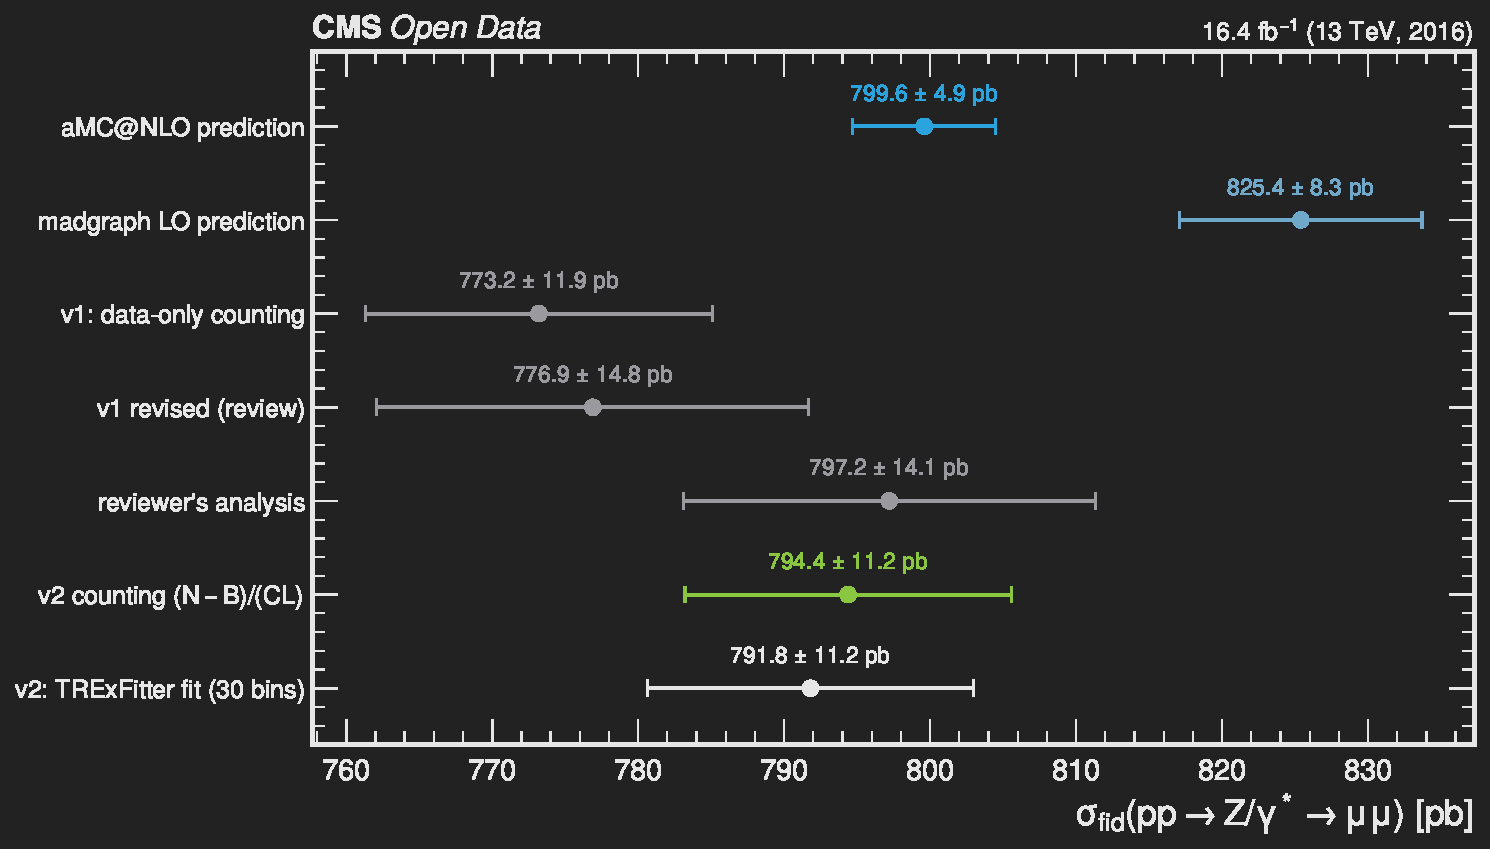
\includegraphics[width=0.97\textwidth]{summary_sigma.pdf}
    \end{column}
    \begin{column}{0.48\textwidth}\tsize
      \begin{tabular}{L{3.6cm}R{2.4cm}}
        \thead quantity & value\\
        \rowcolor{rowA} $\sfid$ (fit, 30 bins) & $791.8 \pm 11.2\pb$\\
        \rowcolor{rowB} $\sfid$ (counting $(N-B)/(CL)$) & \bestcell{$794.4\pb$}\\
        \rowcolor{rowA} $\muZ$ & $0.990\,^{+0.014}_{-0.014}$\\
        \rowcolor{rowB} $\sigma(60<m<120)$, $A=0.4092$ & $1935 \pm 30\pb$\\
        \rowcolor{rowA} $\sigma(m>50)$, $A=0.3947$ & $2006 \pm 31\pb$\\
        \rowcolor{rowB} $C$ (reco / fiducial) & 0.7917\\
        \rowcolor{rowA} aMC@NLO $\sfid^{\mathrm{pred}}$ & $799.6\pb$\\
        \rowcolor{rowB} external reviewer, same volume & $797.2\pb$\\
      \end{tabular}\\[0.3cm]
      \begin{itemize}\footnotesize
        \item Every extraction lands within 1\,\% of the aMC@NLO prediction; the physics is fine.
        \item The 0.03\,\% ``statistical'' uncertainty is misleading: the effective statistical limit is the MC (0.35\,\%).
        \item The counting result is highlighted as the robust number (next slides).
      \end{itemize}
    \end{column}
  \end{columns}
\end{frame}

\begin{frame}{The fit is not robust: $\muZ$ versus fit configuration}
  \tsize
  \begin{tabular}{L{4.4cm}R{2.2cm}R{1.2cm}L{5.2cm}}
    \thead configuration (\texttt{review/fitcheck/}) & $\muZ$ & GoF $p$ & notable pulls (constraints)\\
    \rowcolor{rowA} nominal: 30 $\times$ 2 GeV & $0.9903\,^{+0.0141}_{-0.0138}$ & 0.33 & SigModel +0.5 (0.10), MuonScale (0.11), MuonRes (0.21), Pileup $-$1.5, PDF +1.3, MuonIso $-$1.1\\
    \rowcolor{rowB} 6 $\times$ 10 GeV & $0.9959 \pm 0.0160$ & 0.0009 & MuonIso $-$1.7, PS\_ISR +1.3, PS\_FSR +1.2\\
    \rowcolor{rowA} 1 bin (= counting) & \bestcell{$0.9935$} & -- & grouped total 1.49\,\%\\
    \rowcolor{rowB} 30 bins, no SigModel & $1.0050\,^{+0.0141}_{-0.0137}$ & 0.0014 & \textbf{MuonIso $-$3.0$\sigma$}, QCDScale $-$0.7, MuonScale (0.06)\\
    \rowcolor{rowA} 30 bins, no SigModel, no smoothing & $1.0063\,^{+0.0141}_{-0.0137}$ & 0.0003 & MuonIso $-$3.1$\sigma$, Pileup (0.48), Lumi (0.22)\\
  \end{tabular}\\[0.35cm]
  \begin{itemize}
    \item Spread 0.990--1.006 = $\pm$0.8\,\%, larger than the whole non-lumi systematic (0.77\,\%). In $\sfid$: 792 to 805 pb.
    \item Data show a 3--4\,\% deficit against aMC@NLO at 62--78 GeV. With the powheg template the fit explains it as ``generator''; without it, as an isolation efficiency 1\,\% below tag-and-probe. The data cannot tell which.
    \item 10 M events in 2 GeV bins resolve $10^{-3}$ shape differences: finer than the MC precision of the templates and than their physics content. The resulting constraints are artefacts (\texttt{Lumi} measured by the t$\bar{\mathrm{t}}$ sideband shape).
    \item The counting extraction is insensitive to the lineshape to first order: $C$ is a ratio of the same MC in the same window.
  \end{itemize}
\end{frame}

\begin{frame}{What the fit uses to absorb the low-mass tail}
  \begin{columns}[T]
    \begin{column}{0.52\textwidth}\centering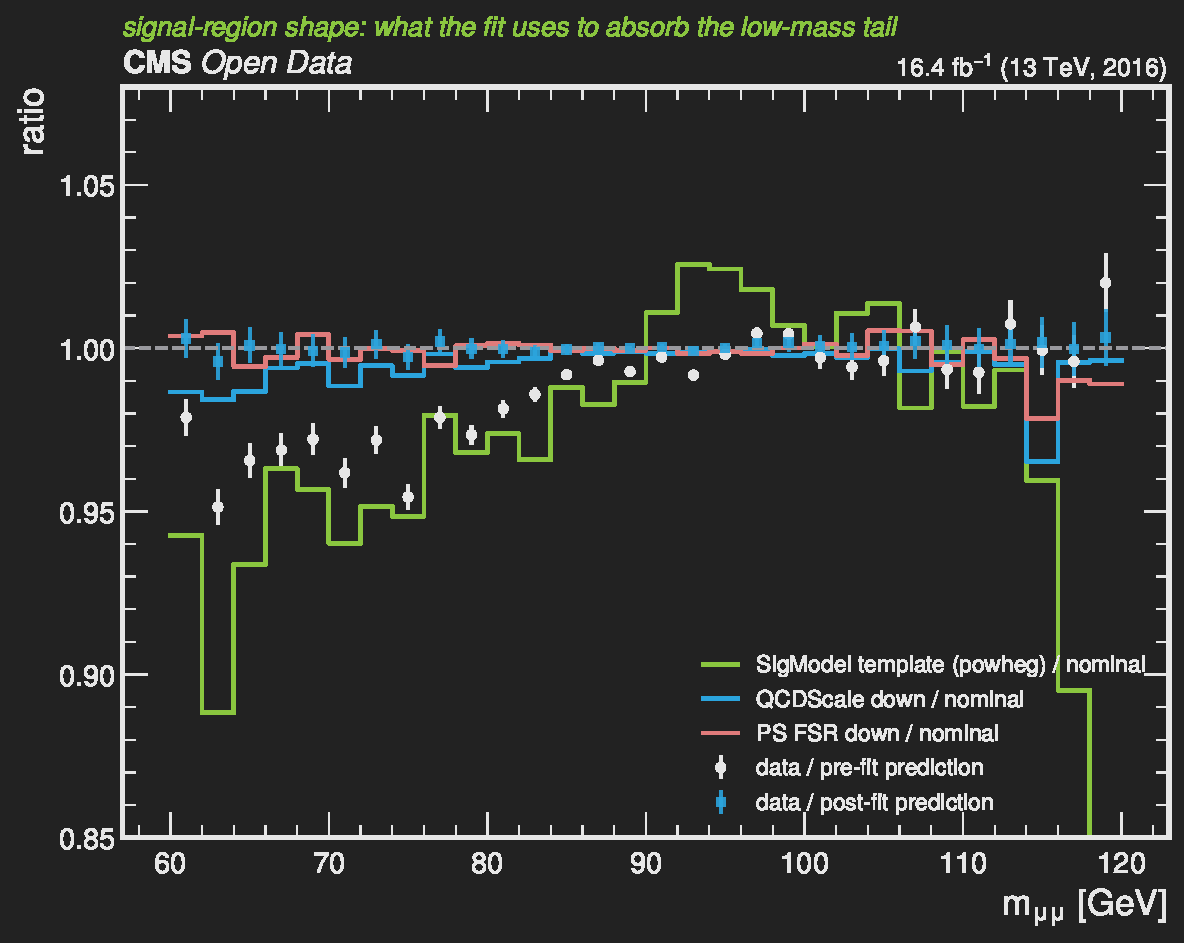
\includegraphics[width=\textwidth]{fit_sigmodel_shape.pdf}\end{column}
    \begin{column}{0.43\textwidth}\small
      \begin{itemize}
        \item Grey: data / pre-fit prediction. 0.95--0.97 for $62<m<78$ GeV, $1.00\pm0.005$ above 86 GeV. Backgrounds are 7\,\% of the first bin and validated by the e$\mu$ region: this is the Z/$\gamma^*$ lineshape (continuum, FSR tail, resolution).
        \item Green: powheg / aMC@NLO. $-$6 to $-$11\,\% at 60--70 GeV, +2.5\,\% at the peak, $-$10\,\% / $-$33\,\% in the last two bins from the $m_{\mathrm{LHE}}<120$ generator cut of the powheg sample (resolution migration). That edge is a phase-space artefact, not modelling.
        \item QCD-scale and PS-FSR variations (blue, red) are flat at the 0.5\,\% level: no other NP can describe the tail.
        \item Blue points: data / post-fit, flat, $p = 0.33$, obtained with SigModel pulled +0.5$\sigma$ and constrained to 0.10.
      \end{itemize}
    \end{column}
  \end{columns}
\end{frame}

\begin{frame}{Nuisance parameters: pulls, constraints, ranking}
  \begin{columns}[T]
    \begin{column}{0.48\textwidth}\centering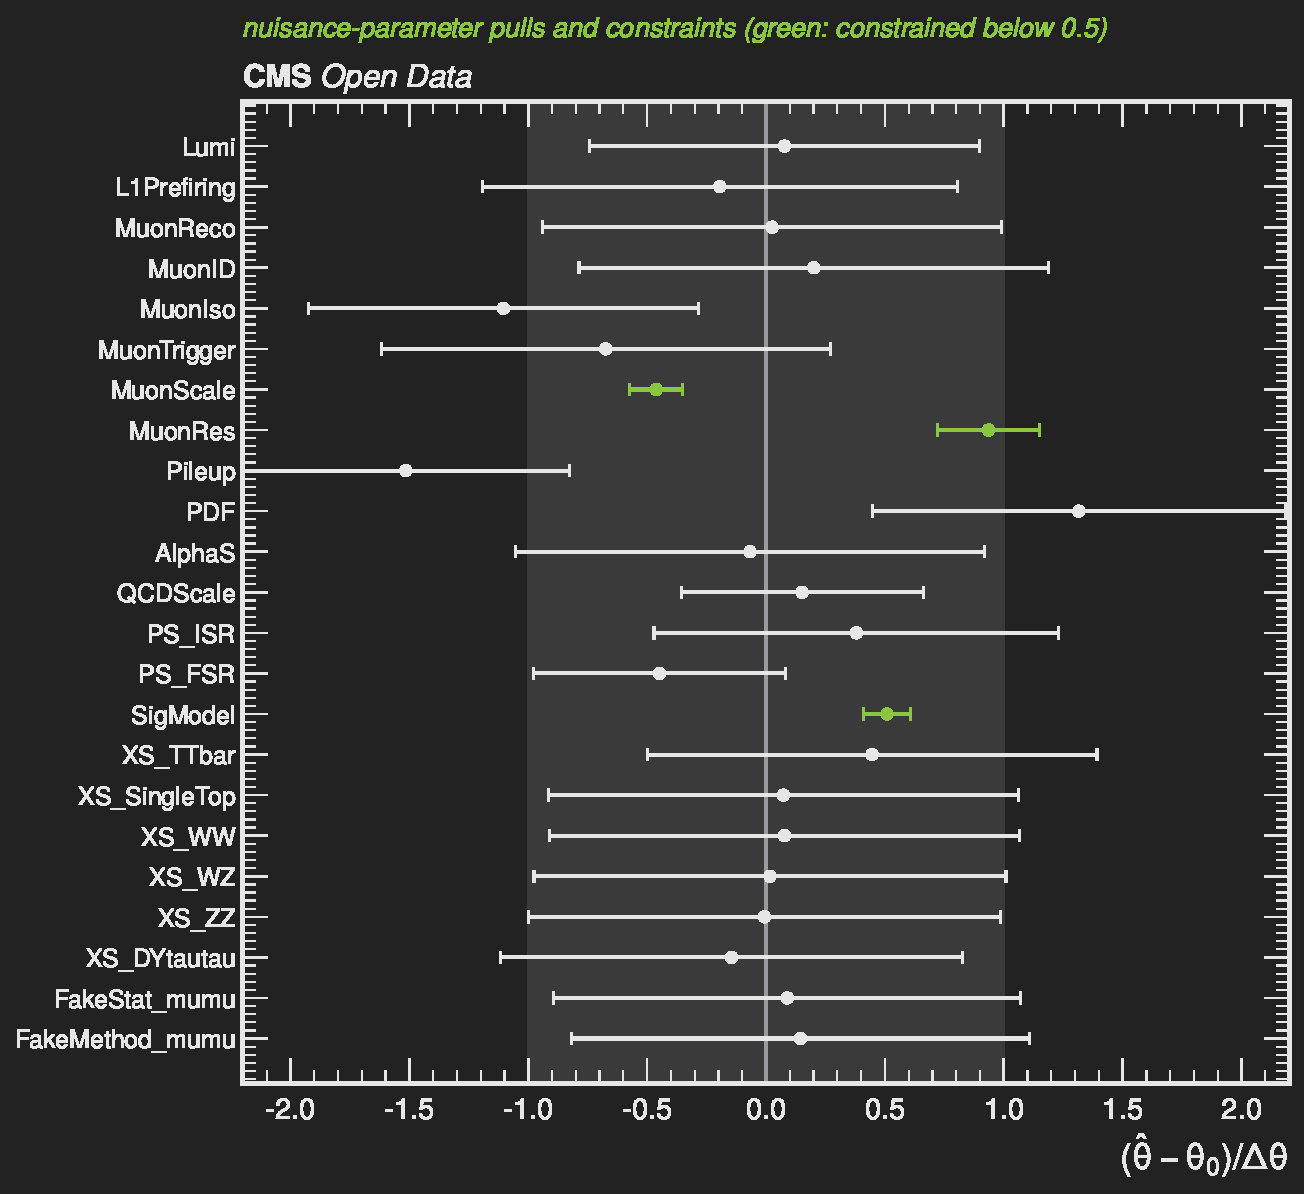
\includegraphics[height=0.76\textheight]{fit_pulls.pdf}\end{column}
    \begin{column}{0.5\textwidth}\centering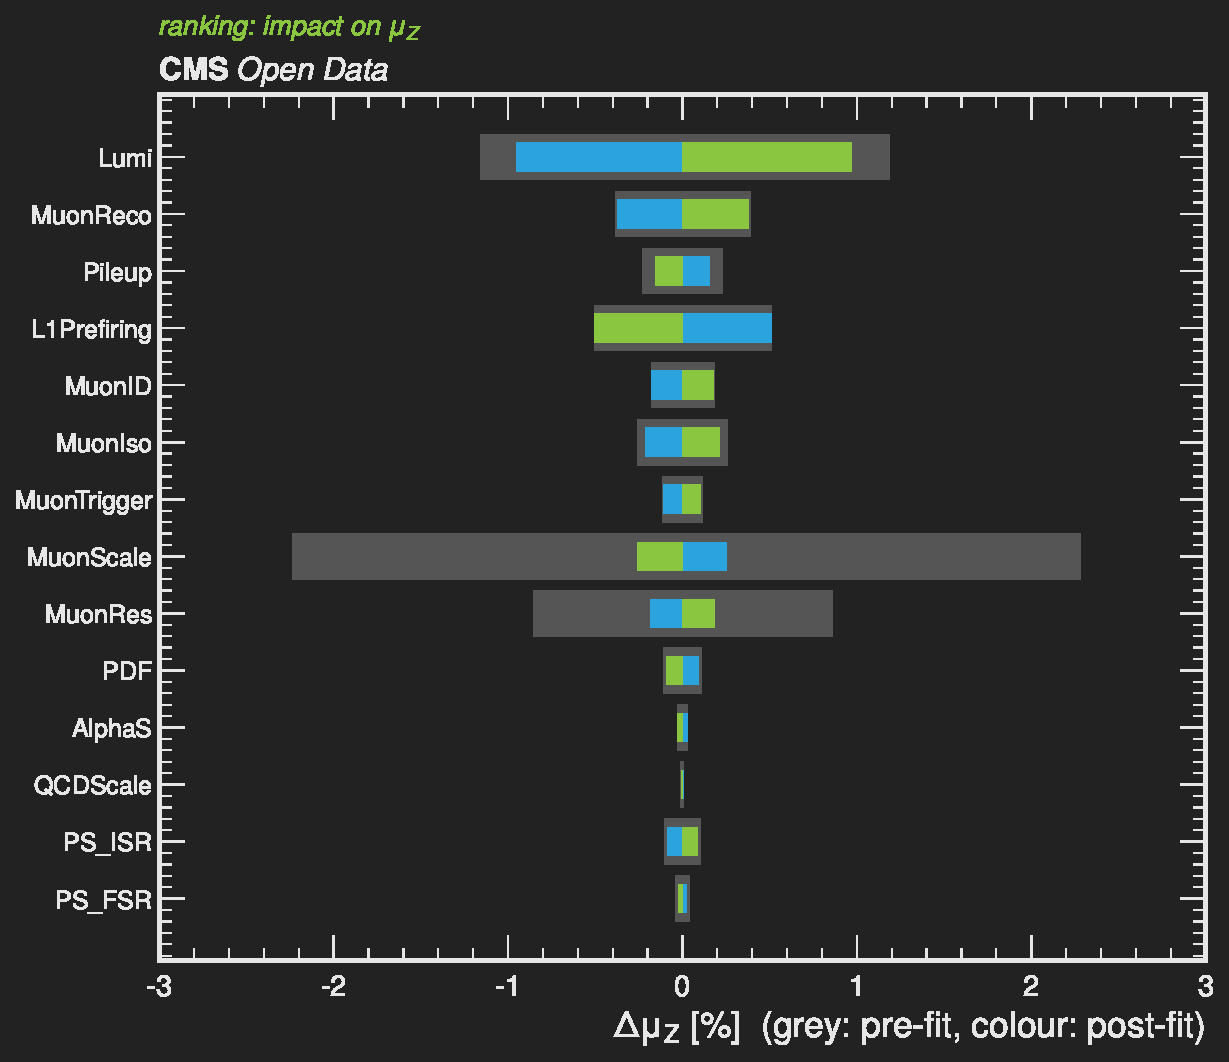
\includegraphics[height=0.52\textheight]{fit_ranking.pdf}\\
      \begin{minipage}{0.95\textwidth}\footnotesize
        Pre-fit impacts (grey) of MuonScale (2.3\,\%) and SigModel (2.8\,\%) shrink to 0.25--0.3\,\% post-fit: the 2 GeV shape ``measures'' them. \texttt{Pileup} is pulled towards \emph{less} pileup while $N_{PV}$ asks for more (F6): the mass shape carries no pileup information.
      \end{minipage}
    \end{column}
  \end{columns}
\end{frame}

\begin{frame}{Uncertainty budget (as quoted) and what the review changes}
  \tsize
  \begin{columns}[T]
    \begin{column}{0.5\textwidth}
      \begin{tabular}{L{3.0cm}R{1.5cm}L{2.2cm}}
        \thead group & impact on $\muZ$ & review\\
        \rowcolor{rowA} luminosity & 1.16\,\% & quote 1.20\,\% (F5)\\
        \rowcolor{rowB} L1 prefiring & 0.51\,\% & ok\\
        \rowcolor{rowA} muon efficiency & 0.50\,\% & F8: +0.35\,\%?\\
        \rowcolor{rowB} signal modelling & 0.36\,\% & F3/F4: +0.7\,\%\\
        \rowcolor{rowA} MC statistics & 0.35\,\% & inherent\\
        \rowcolor{rowB} muon momentum & 0.27\,\% & calibration used twice\\
        \rowcolor{rowA} pileup & 0.16\,\% & F6 profile\\
        \rowcolor{rowB} backgrounds & 0.09\,\% & ok\\
        \rowcolor{rowA} fakes & 0.05\,\% & ok\\
        \rowcolor{rowB} statistical & 0.03\,\% & ok\\
        \rowcolor{rowA} \textbf{total} & \textbf{1.40\,\%} & $\approx$ 1.6\,\% after fixes\\
      \end{tabular}
    \end{column}
    \begin{column}{0.48\textwidth}\small
      \begin{itemize}
        \item MC statistics per mass bin is 1.7$\times$ the data statistics: the 30 gammas are pulled up to 1.3$\sigma$ and constrained to 0.6. The fit is MC-limited, not data-limited.
        \item A lineshape-model term of $\pm$0.7\,\% (half the spread of the fit variants) should be added until the 62--78 GeV deficit is understood.
        \item \texttt{MuonReco}: docs say 0.4\,\% per muon (v1 used 0.8\,\% per event), the fit applies 0.4\,\% per event.
        \item The acceptance uncertainty (0.61\,\%: PDF 0.52, scales 0.32) is correctly kept outside $\sfid$ and added only for $\sigma_{\mathrm{tot}}$.
      \end{itemize}
    \end{column}
  \end{columns}
\end{frame}

% ================================================================= 2. e-mu region
\divider{The e$\mu$ control region}

\begin{frame}{The problem as plotted: +9\,\% in the opposite-sign e$\mu$ region}
  \begin{columns}[T]
    \begin{column}{0.33\textwidth}\centering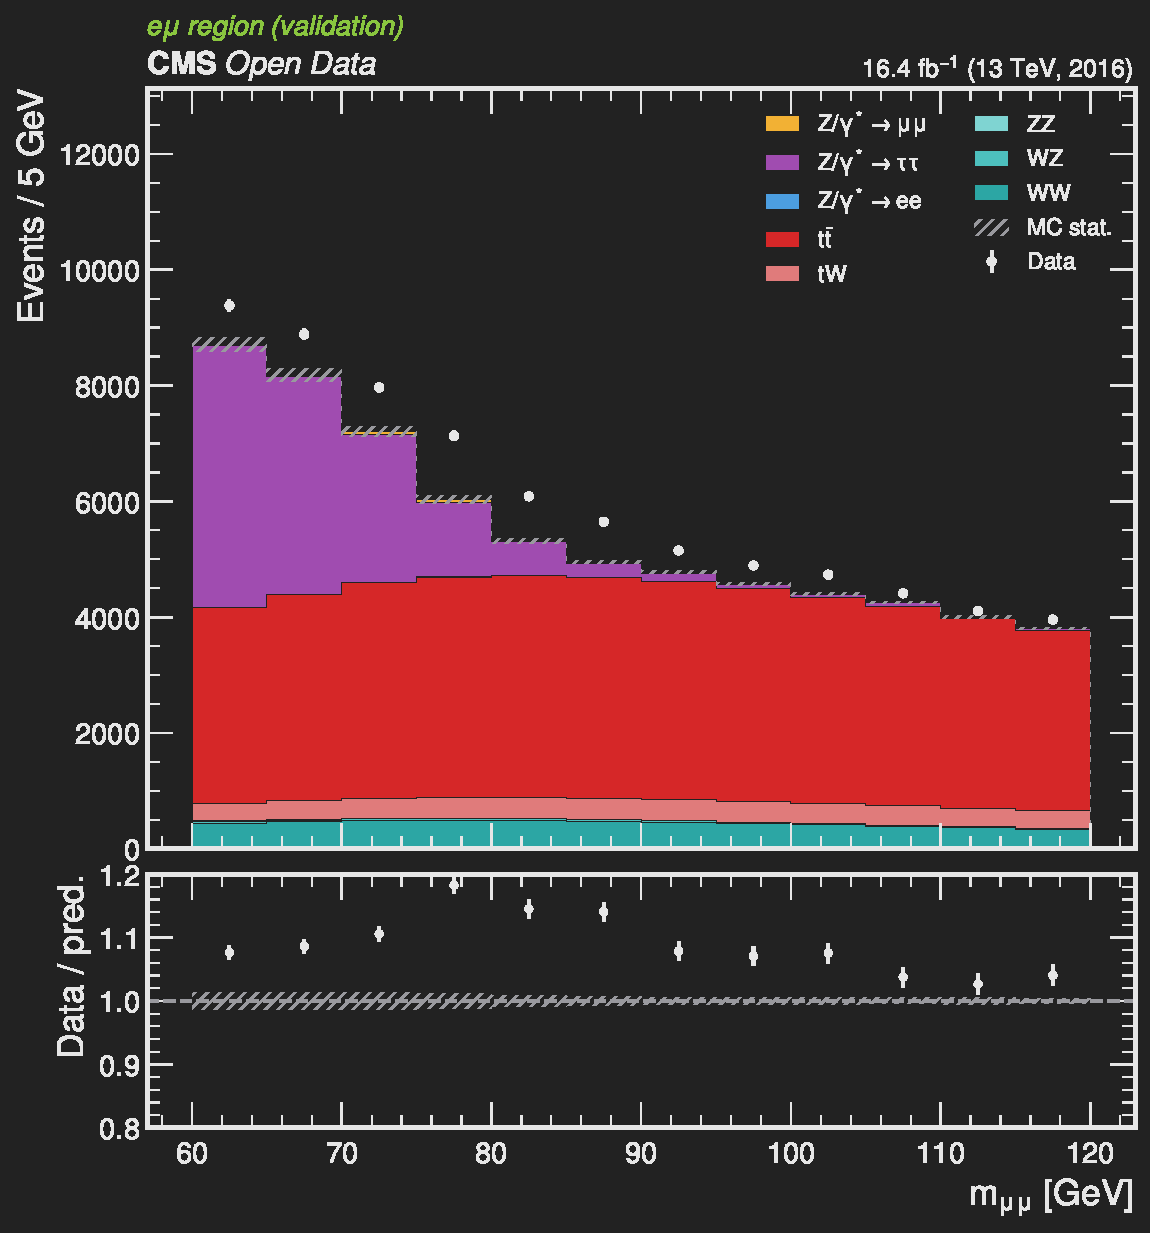
\includegraphics[width=0.9\textwidth]{cr_mass.pdf}\fcap{$m_{e\mu}$: excess at 75--90 GeV}\end{column}
    \begin{column}{0.33\textwidth}\centering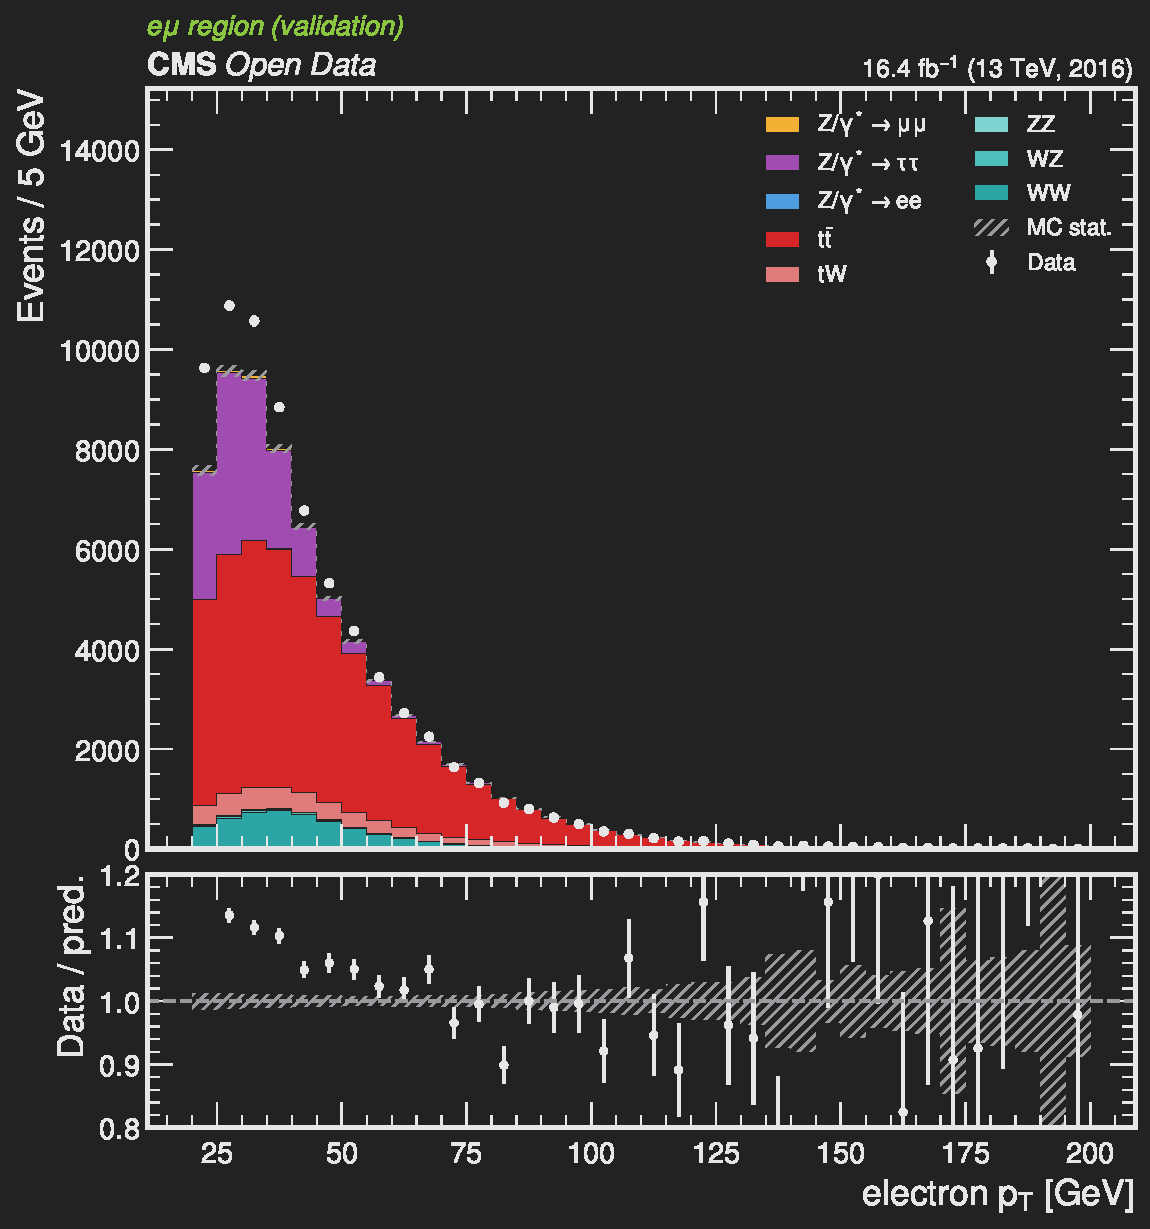
\includegraphics[width=0.9\textwidth]{cr_pt_el.pdf}\fcap{electron $p_T$: 1.27 at 20--25 GeV, 1.02 above 55 GeV}\end{column}
    \begin{column}{0.33\textwidth}\centering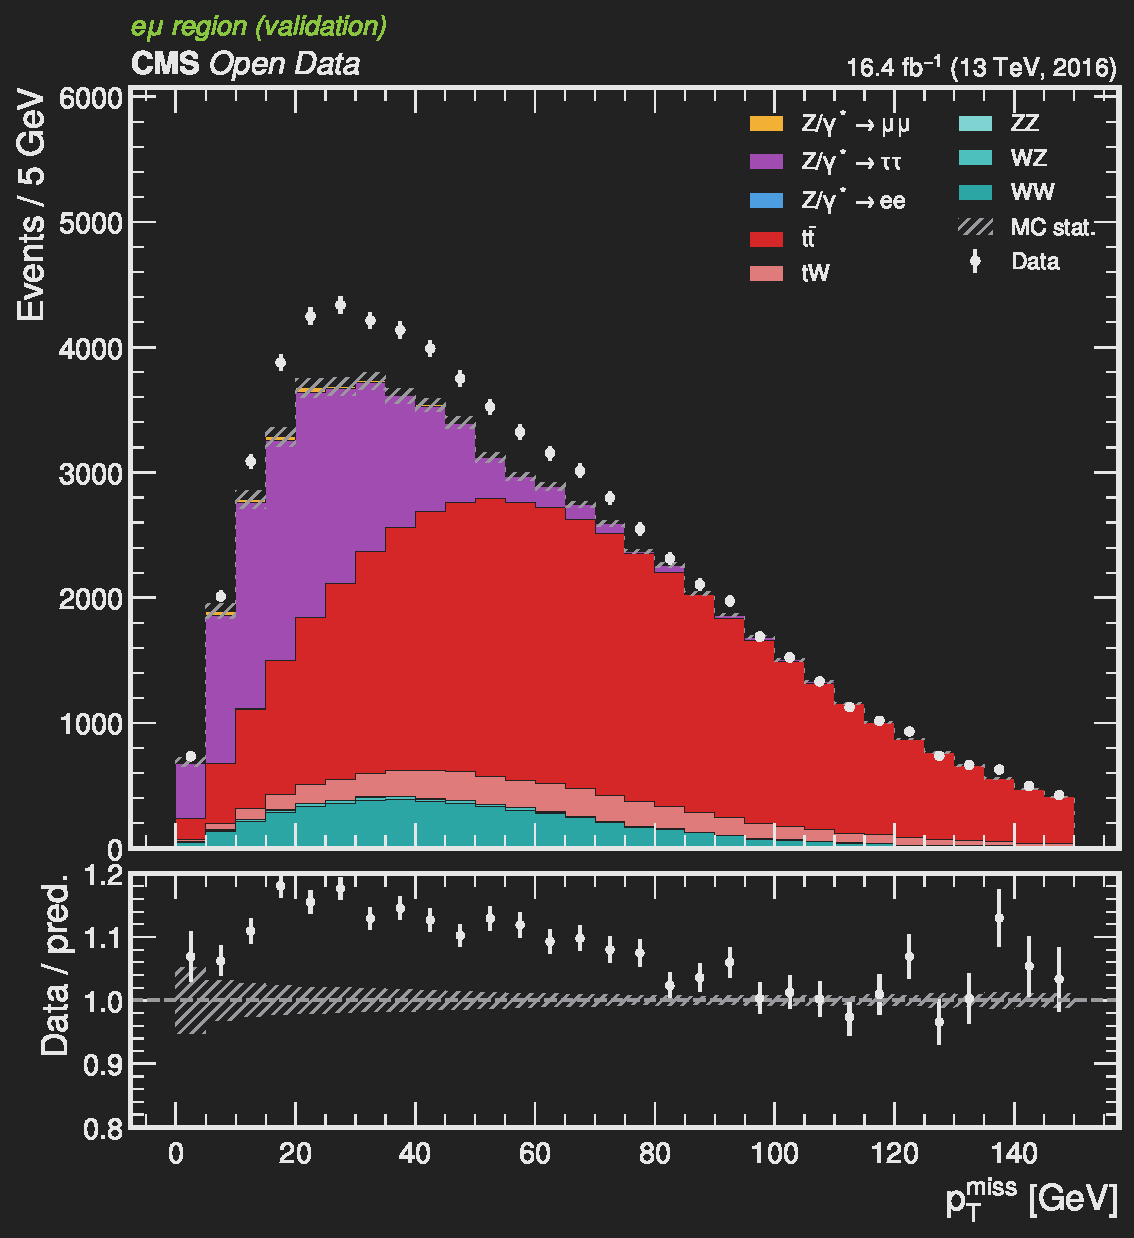
\includegraphics[width=0.9\textwidth]{cr_met.pdf}\fcap{$\met$: excess at 10--50 GeV}\end{column}
  \end{columns}
  \vspace{0.1cm}\footnotesize
  Low electron $p_T$, no jets (next slide), moderate $\met$, visible mass just above Z$\to\tau\tau\to$e$\mu$: the signature of a \textbf{non-prompt electron} next to a real W/Z muon, not a normalisation problem of t$\bar{\mathrm{t}}$ or WW (which populate $\geq 2$ jets and agree to 1\,\%).
\end{frame}

\begin{frame}{The explanation: the prompt-only MC filter removes a whole background}
  \centering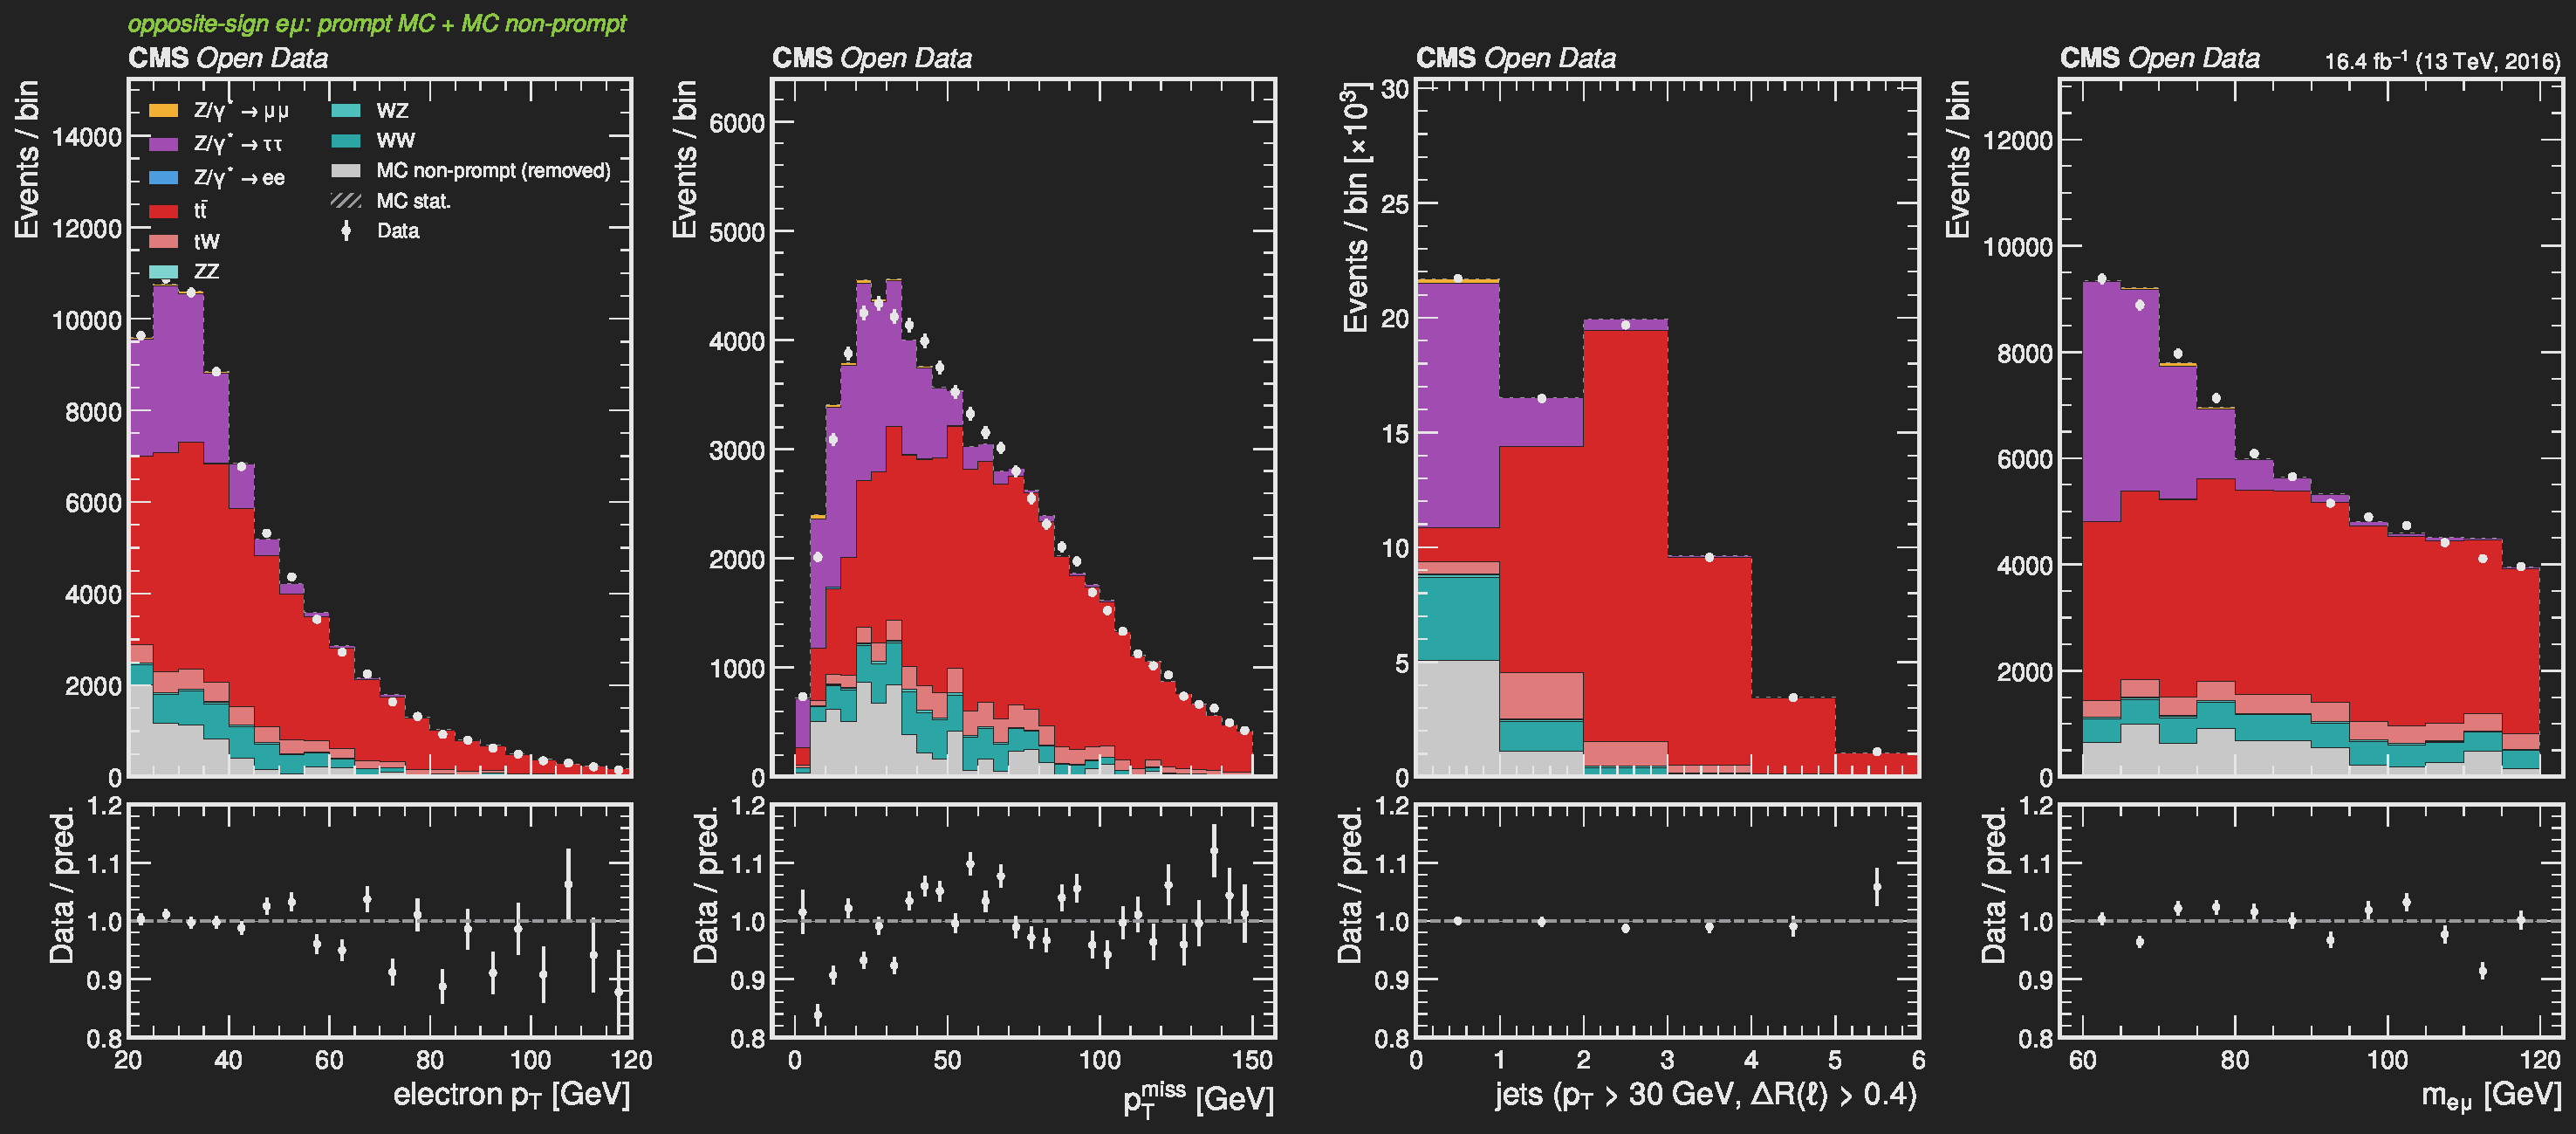
\includegraphics[width=0.92\textwidth]{emu_os_with_nonprompt.pdf}
  \vspace{-0.05cm}\footnotesize
  \texttt{histograms.fill\_chunk} keeps MC events only if both leptons have \texttt{genPartFlav} $\in\{1,15\}$. In the SR the fake factor replaces the removed muons; in the e$\mu$ region nothing replaces the removed electrons. Grey = what was removed (review pass over the skims), now included: data/MC = 0.996, flat in every variable.
\end{frame}

\begin{frame}{e$\mu$ accounting: MC composition and the same-sign cross-check}
  \begin{columns}[T]
    \begin{column}{0.5\textwidth}\tsize
      \begin{tabular}{L{4.6cm}R{1.5cm}}
        \thead opposite-sign e$\mu$ & events\\
        \rowcolor{rowA} data & 72\,357\\
        \rowcolor{rowB} prompt-prompt MC (as in v2) & 66\,232\\
        \rowcolor{rowA} \textbf{data $-$ prompt MC} & \textbf{6\,125 (+9.2\,\%)}\\
        \rowcolor{rowB} MC non-prompt, removed: W+jets 3\,412, Z$\to\mu\mu$+$\gamma$ 1\,344, Z$\to\mu\mu$ other 660, Z$\to\tau\tau$ $\tau_h\to$e 627, top 328, VV 27 & \bestcell{6\,412}\\
        \rowcolor{rowA} data / (prompt + non-prompt) & \bestcell{0.996}\\
        \thead same-sign e$\mu$ (new region) & events\\
        \rowcolor{rowA} data & 6\,718\\
        \rowcolor{rowB} prompt-prompt MC & 1\,039\\
        \rowcolor{rowA} charge-symmetric non-prompt (data-driven) & 5\,679\\
        \rowcolor{rowB} + OS-only ($\tau_h\to$e, b$\to$e from MC) & 955\\
        \rowcolor{rowA} SS-based prediction for the OS excess & \bestcell{6\,630}\\
      \end{tabular}
    \end{column}
    \begin{column}{0.48\textwidth}\centering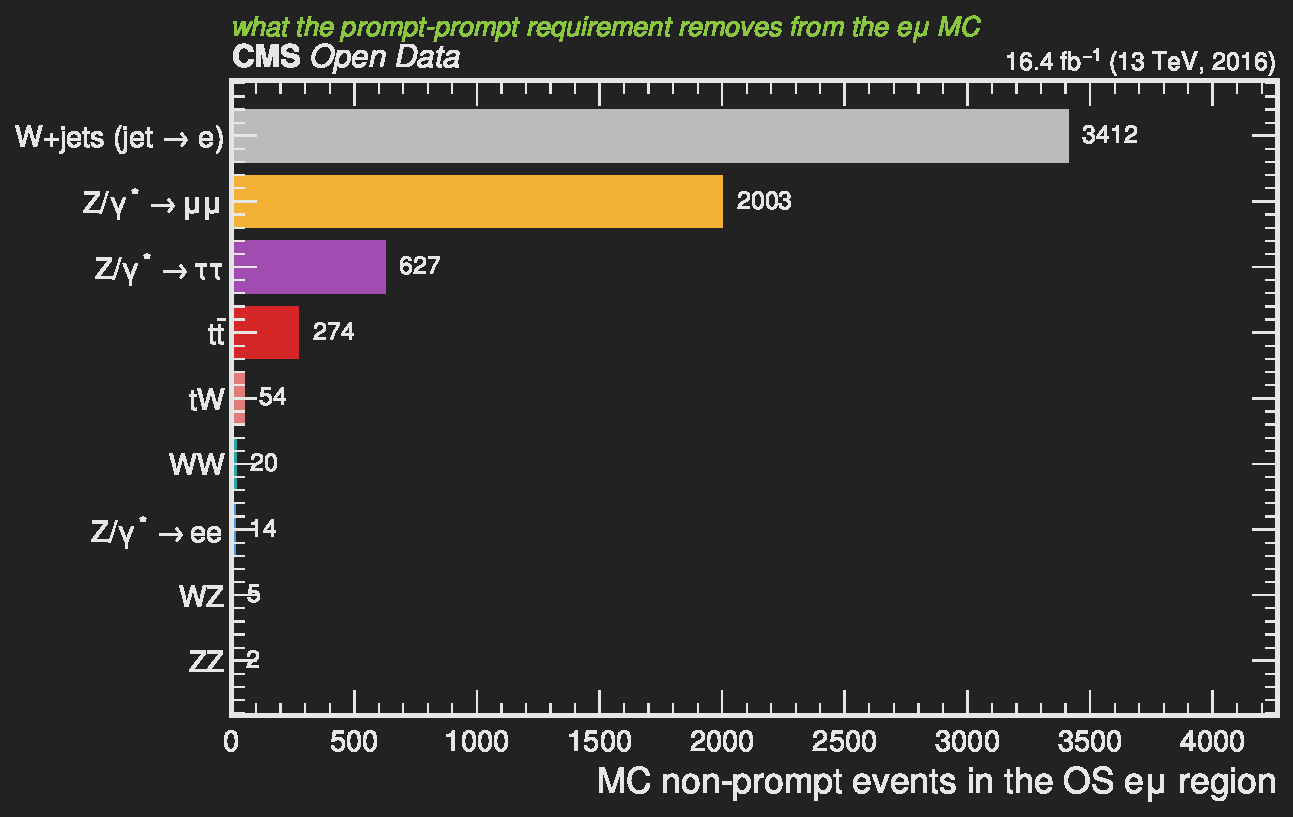
\includegraphics[width=\textwidth]{emu_nonprompt_composition.pdf}
      \begin{minipage}{0.95\textwidth}\footnotesize
        Consequences: none for $\sfid$ (the region is \texttt{VALIDATION}). But \texttt{--emu-control} with $\mu_{\mathrm{top}}$ would absorb 9\,\% of non-prompt events into t$\bar{\mathrm{t}}$: keep it a validation region until the non-prompt component is included. Electron scale factors would move the prediction the \emph{wrong} way (0.97--0.99).
      \end{minipage}
    \end{column}
  \end{columns}
\end{frame}

% ================================================================= 3. MET
\divider{$\met$ in the signal region}

\begin{frame}{$\met$: data broader than MC, and why}
  \begin{columns}[T]
    \begin{column}{0.30\textwidth}\centering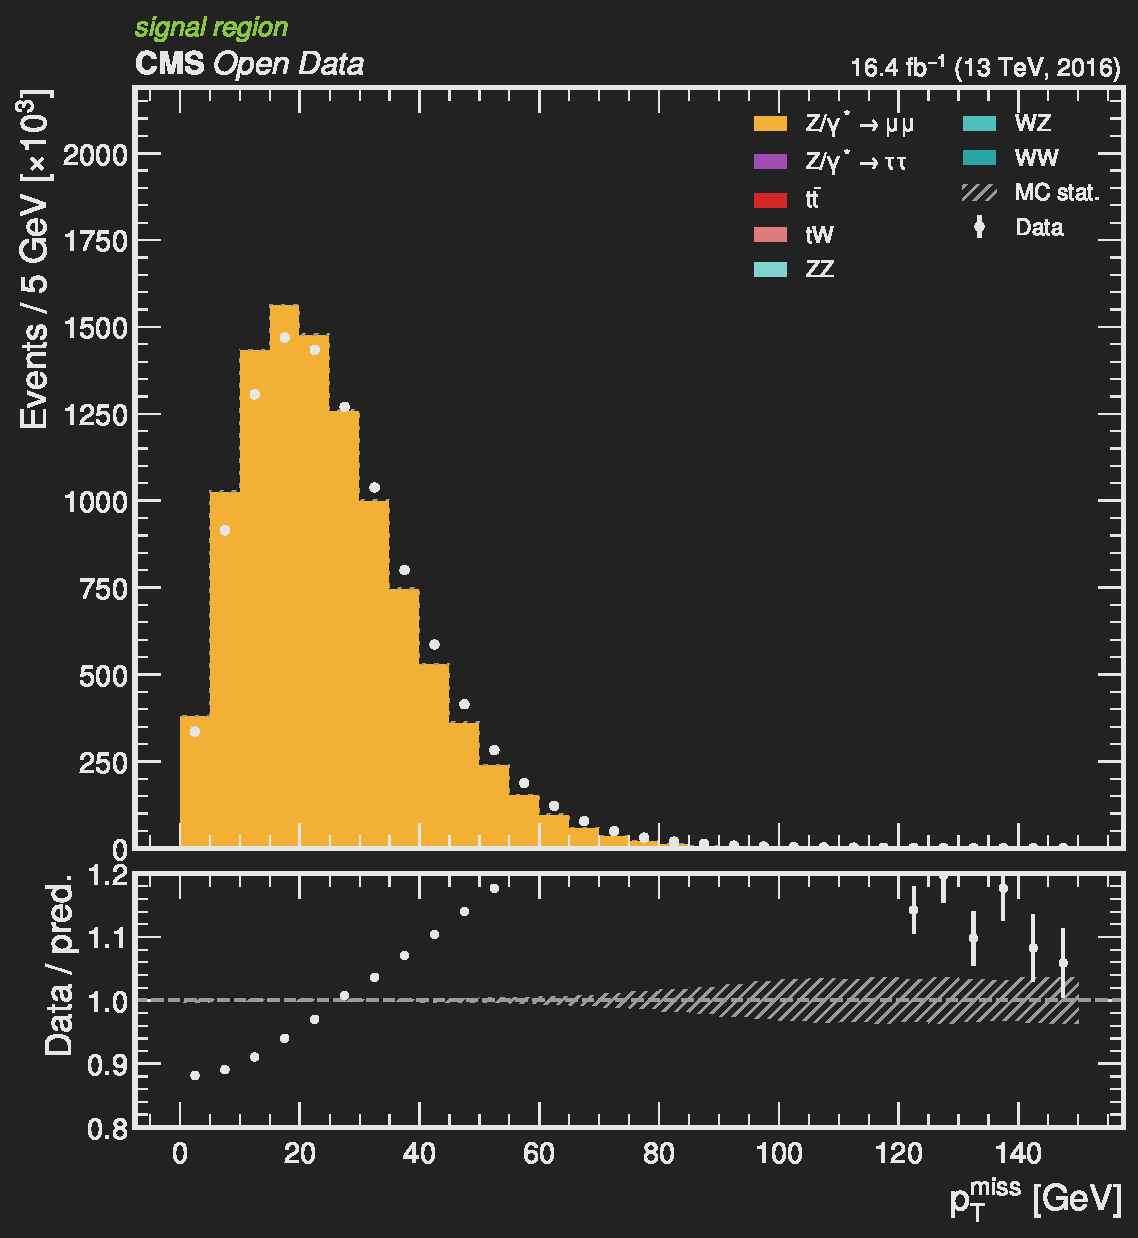
\includegraphics[height=0.42\textheight]{sr_met.pdf}\fcap{PF $\met$ in the SR: mean 26.5 (data) vs 25.1 GeV (MC)}\end{column}
    \begin{column}{0.66\textwidth}\centering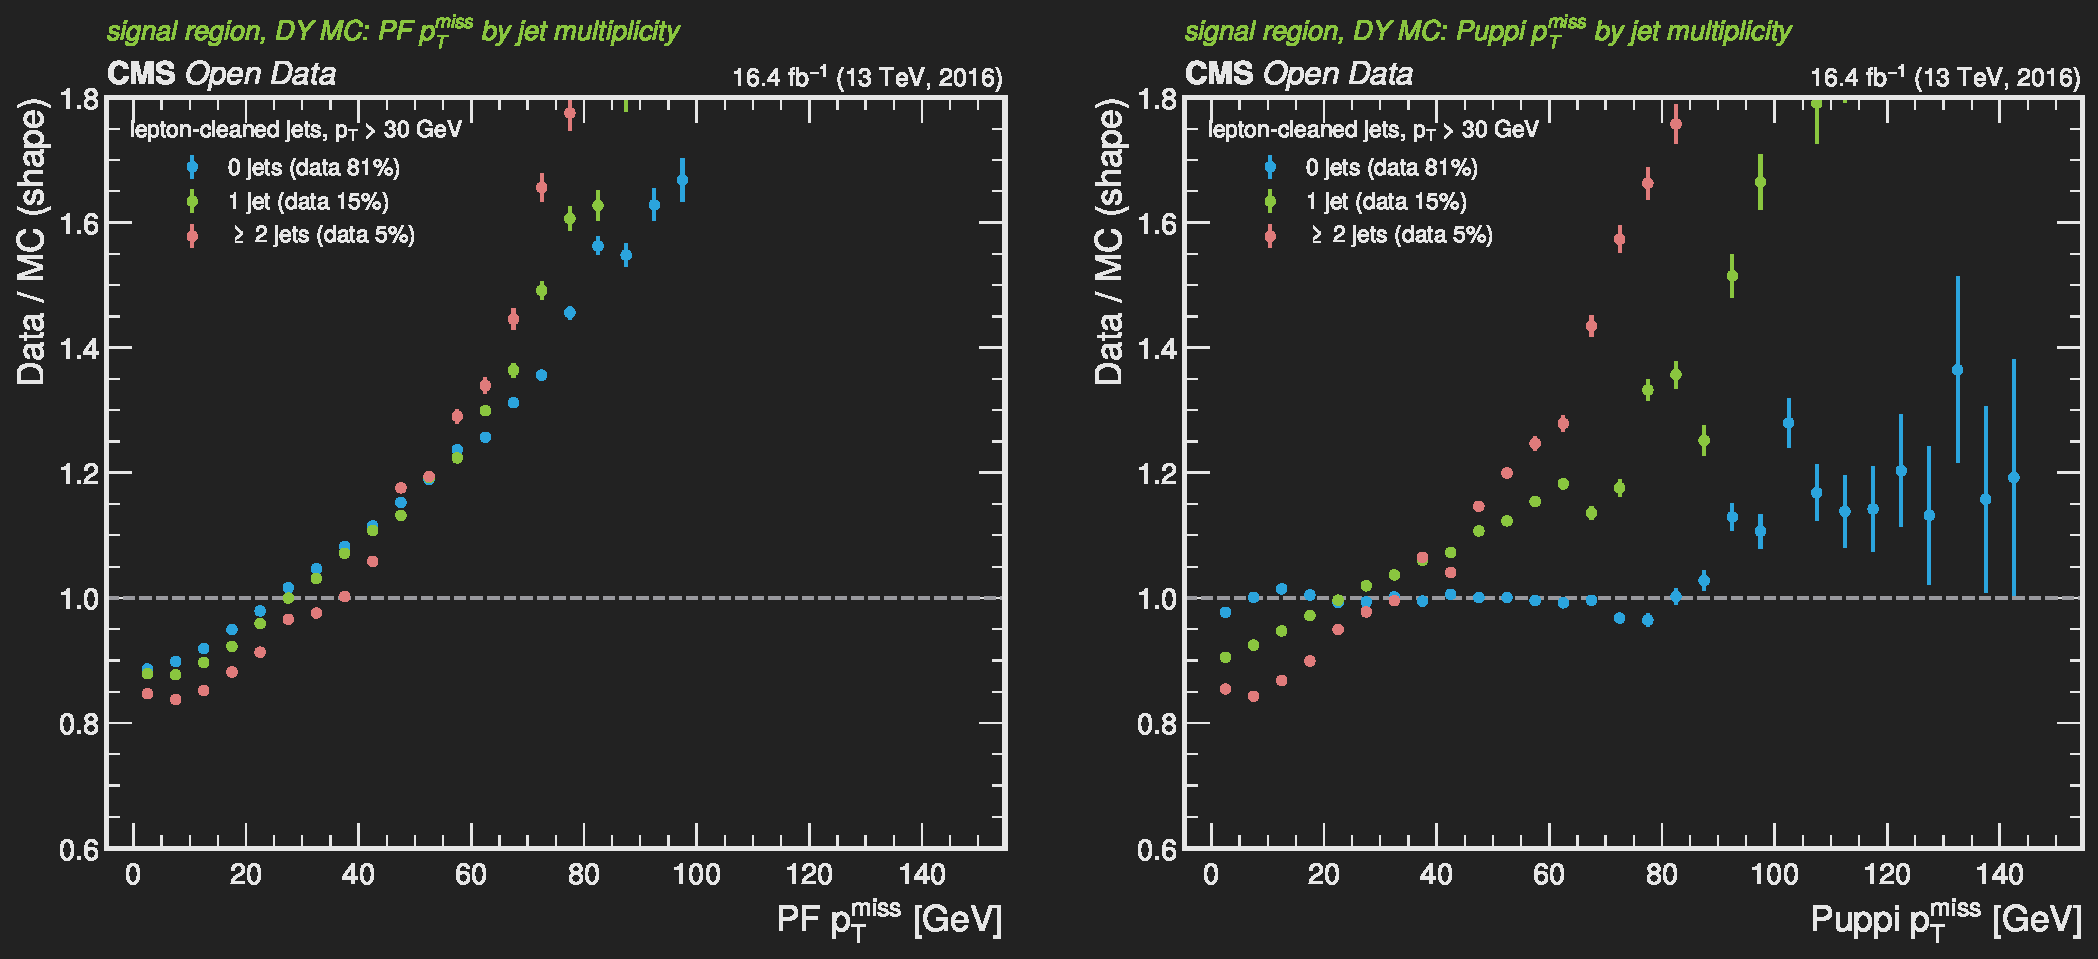
\includegraphics[height=0.42\textheight]{sr_met_by_jets.pdf}\fcap{data/MC shape by lepton-cleaned jet multiplicity: PF (left) and Puppi (right)}\end{column}
  \end{columns}
  \footnotesize
  \begin{itemize}
    \item Z$\to\mu\mu$ has no genuine $\met$: this is a \textbf{resolution} difference. Puppi $\met$ in 0-jet events (81\,\% of the SR) agrees to $<1$\,\% in every bin.
    \item The residual grows with the number of jets for PF and Puppi alike: MC jets are not JER-smeared (NanoAOD MC, no smearing applied), so the recoil is too well measured.
    \item PF $\met$ additionally worsens with pileup (next slide): pileup / unclustered energy, and the profile of F6. Z $p_T$ mismodelling at low $p_T$ (0.83 at 0--5 GeV) adds to it.
    \item $\met$ is not used in the selection or the fit: \textbf{no effect} on $\sfid$. If ever cut on: JER smearing or Puppi $\met$, plus \texttt{MET\_Unclustered}.
  \end{itemize}
\end{frame}

\begin{frame}{Pileup: the profile is about 4\,\% too low}
  \begin{columns}[T]
    \begin{column}{0.36\textwidth}\centering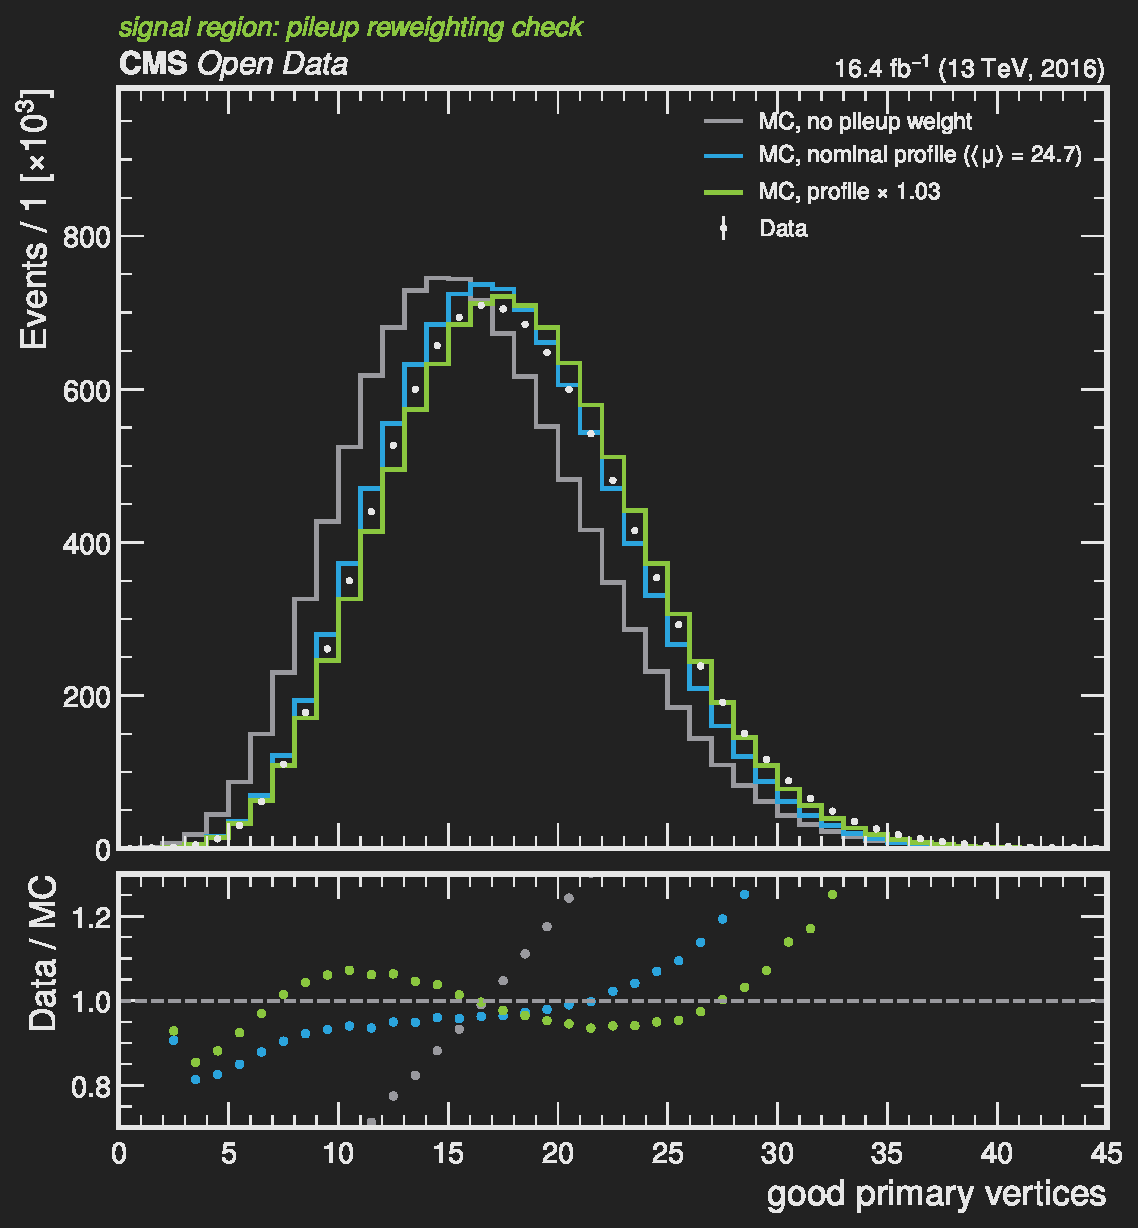
\includegraphics[width=\textwidth]{sr_npv_pileup_check.pdf}\end{column}
    \begin{column}{0.36\textwidth}\centering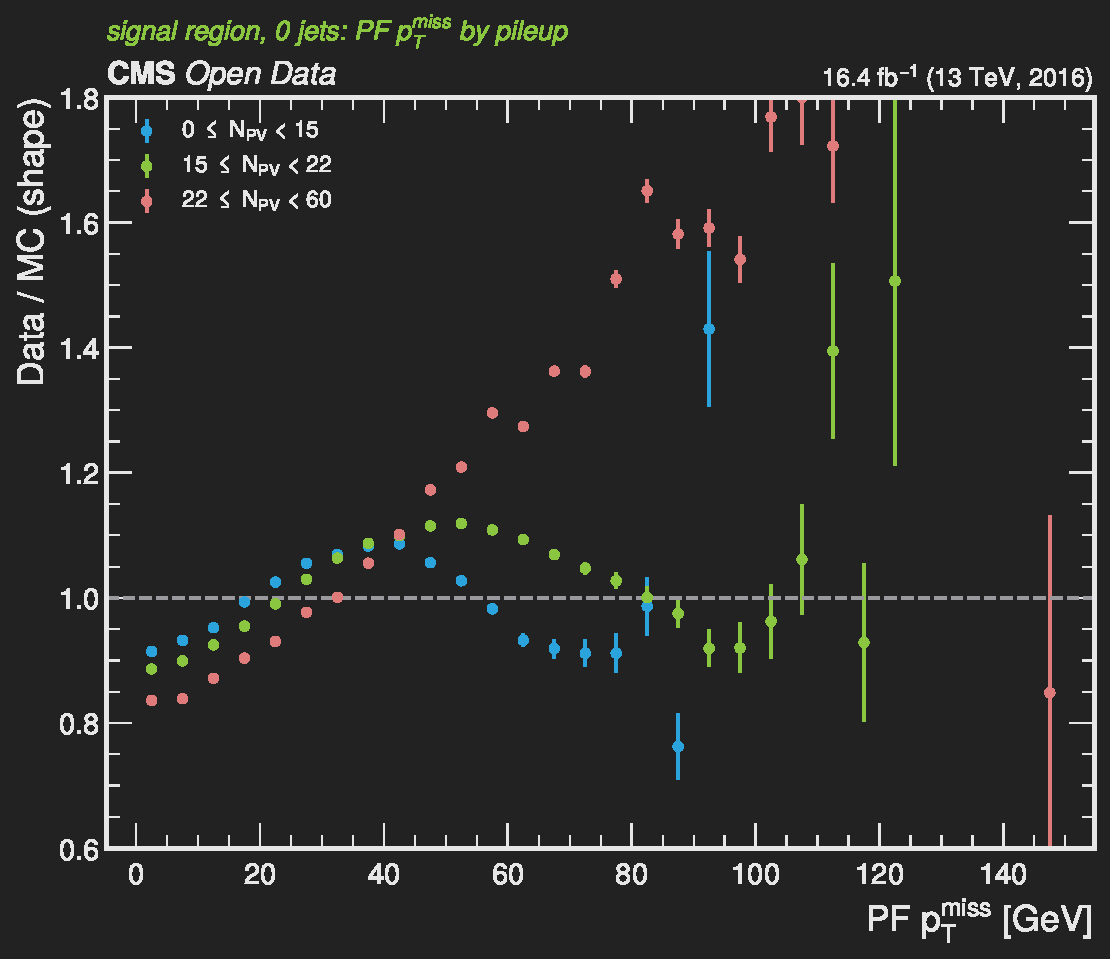
\includegraphics[width=0.95\textwidth]{sr_met_by_pileup.pdf}\end{column}
    \begin{column}{0.23\textwidth}\footnotesize
      \begin{tabular}{L{1.6cm}R{1.0cm}}
        \thead & $\langle N_{PV}\rangle$\\
        \rowcolor{rowA} data & 18.22\\
        \rowcolor{rowB} MC, no weight & 16.26\\
        \rowcolor{rowA} MC, nominal & 17.72\\
        \rowcolor{rowB} era G / H & 17.7 / 18.7\\
      \end{tabular}\\[0.2cm]
      MC: $N_{PV} = 2.16 + 0.63\,N_{\mathrm{true}}$, so data want $\langle N_{\mathrm{true}}\rangle \approx 25.6$ vs 24.6 after reweighting.
    \end{column}
  \end{columns}
  \footnotesize
  The profile from the per-lumisection \texttt{avgpu} (69.2/80 scaling) lacks the bunch-to-bunch spread and is $\sim$1 interaction low. Effect on $\sfid$ $\le 0.05$\,\% (isolation SF measured in data, flat in $N_{PV}$ to 0.5\,\%). The fit's \texttt{Pileup} pull ($-$1.5$\sigma$, towards less pileup) contradicts this: it is template noise, not a measurement.
\end{frame}

% ================================================================= 4. strategy
\divider{Analysis strategy and inputs}

\begin{frame}{Strategy of the v2 measurement}
  \centering
  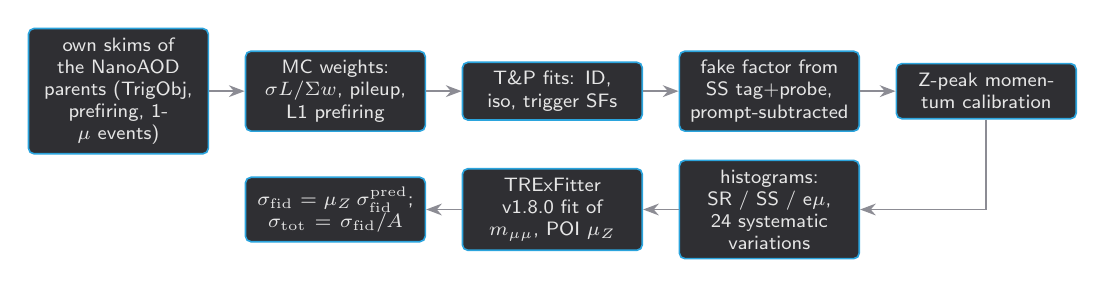
\begin{tikzpicture}[node distance=0.35cm and 0.45cm, every node/.style={font=\scriptsize},
      box/.style={draw=primary, rounded corners=2pt, text=body, fill=rowB, minimum height=0.7cm, text width=2.05cm, align=center, line width=0.6pt},
      arr/.style={-{Stealth[length=2mm]}, draw=rule, line width=0.6pt}]
    \node[box] (skim) {own skims of the NanoAOD parents (TrigObj, prefiring, 1-$\mu$ events)};
    \node[box, right=of skim] (w) {MC weights: $\sigma L/\Sigma w$, pileup, L1 prefiring};
    \node[box, right=of w] (tnp) {T\&P fits: ID, iso, trigger SFs};
    \node[box, right=of tnp] (ff) {fake factor from SS tag+probe, prompt-subtracted};
    \node[box, right=of ff] (mom) {Z-peak momentum calibration};
    \node[box, below=of ff] (hist) {histograms: SR / SS / e$\mu$, 24 systematic variations};
    \node[box, left=of hist] (trex) {TRExFitter v1.8.0 fit of $m_{\mu\mu}$, POI $\muZ$};
    \node[box, left=of trex] (xs) {$\sfid = \muZ\,\sfid^{\mathrm{pred}}$; $\sigma_{\mathrm{tot}} = \sfid/A$};
    \draw[arr] (skim) -- (w); \draw[arr] (w) -- (tnp); \draw[arr] (tnp) -- (ff); \draw[arr] (ff) -- (mom);
    \draw[arr] (mom) |- (hist); \draw[arr] (hist) -- (trex); \draw[arr] (trex) -- (xs);
  \end{tikzpicture}
  \vspace{0.15cm}\footnotesize
  \begin{columns}[T]
    \begin{column}{0.5\textwidth}
      \textbf{Selection (signal region)}
      \begin{itemize}\scriptsize
        \item \texttt{HLT\_IsoMu24 || HLT\_IsoTkMu24}, MET filters, $N_{PV}\ge1$
        \item exactly two tight muons (\texttt{tightId}, iso $<0.15$, $|d_{xy}|<0.2$, $|d_z|<0.5$ cm), $p_T > 26/20$, $|\eta|<2.4$, $\geq 1$ trigger-matched, opposite sign
        \item FSR-recovered $60 < m_{\mu\mu} < 120$ GeV; 30 bins of 2 GeV
      \end{itemize}
    \end{column}
    \begin{column}{0.48\textwidth}
      \textbf{Fiducial volume and normalisation}
      \begin{itemize}\scriptsize
        \item dressed muons ($\Delta R<0.1$), $p_T > 26/20$, $|\eta|<2.4$, $60<m<120$ GeV; $C = 0.7917$, $A_{60\text{--}120} = 0.4092$ (aMC@NLO)
        \item $\sigma(Z/\gamma^*\to\ell\ell, m>50) = 6077.22/3$ pb, $L = 16393.381$ pb$^{-1}$ (normtag)
        \item backgrounds: Z$\to\tau\tau$, t$\bar{\mathrm{t}}$, tW, WW, WZ, ZZ from MC (0.6\,\%), non-prompt from data (0.035\,\%)
      \end{itemize}
    \end{column}
  \end{columns}
\end{frame}

\begin{frame}{Signal region: mass spectrum}
  \begin{columns}[T]
    \begin{column}{0.44\textwidth}\centering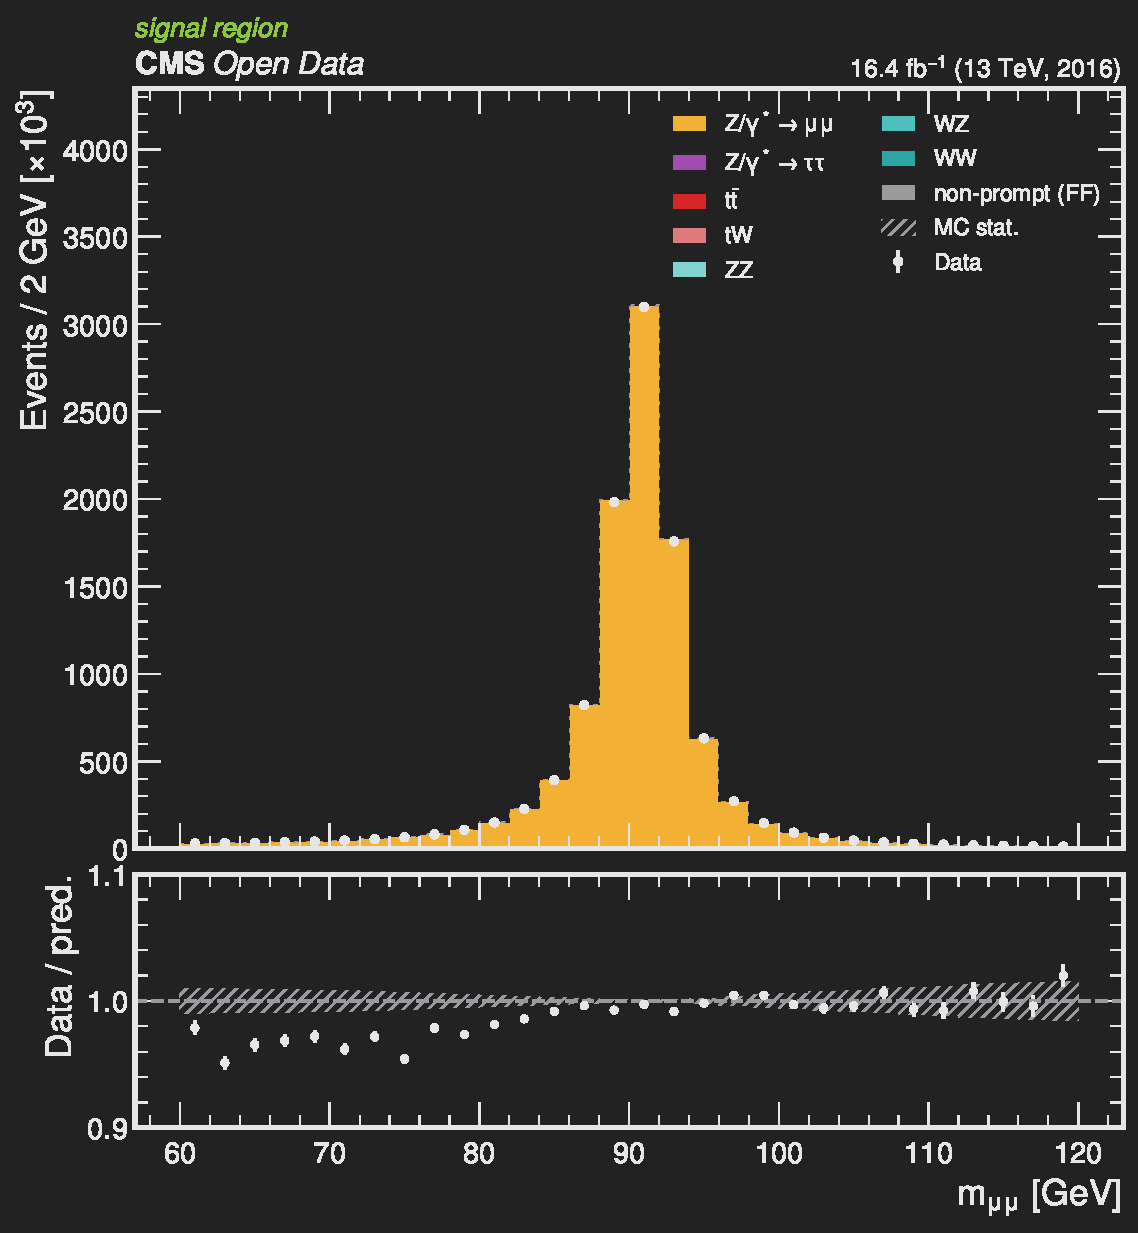
\includegraphics[height=0.7\textheight]{sr_mass.pdf}\end{column}
    \begin{column}{0.44\textwidth}\centering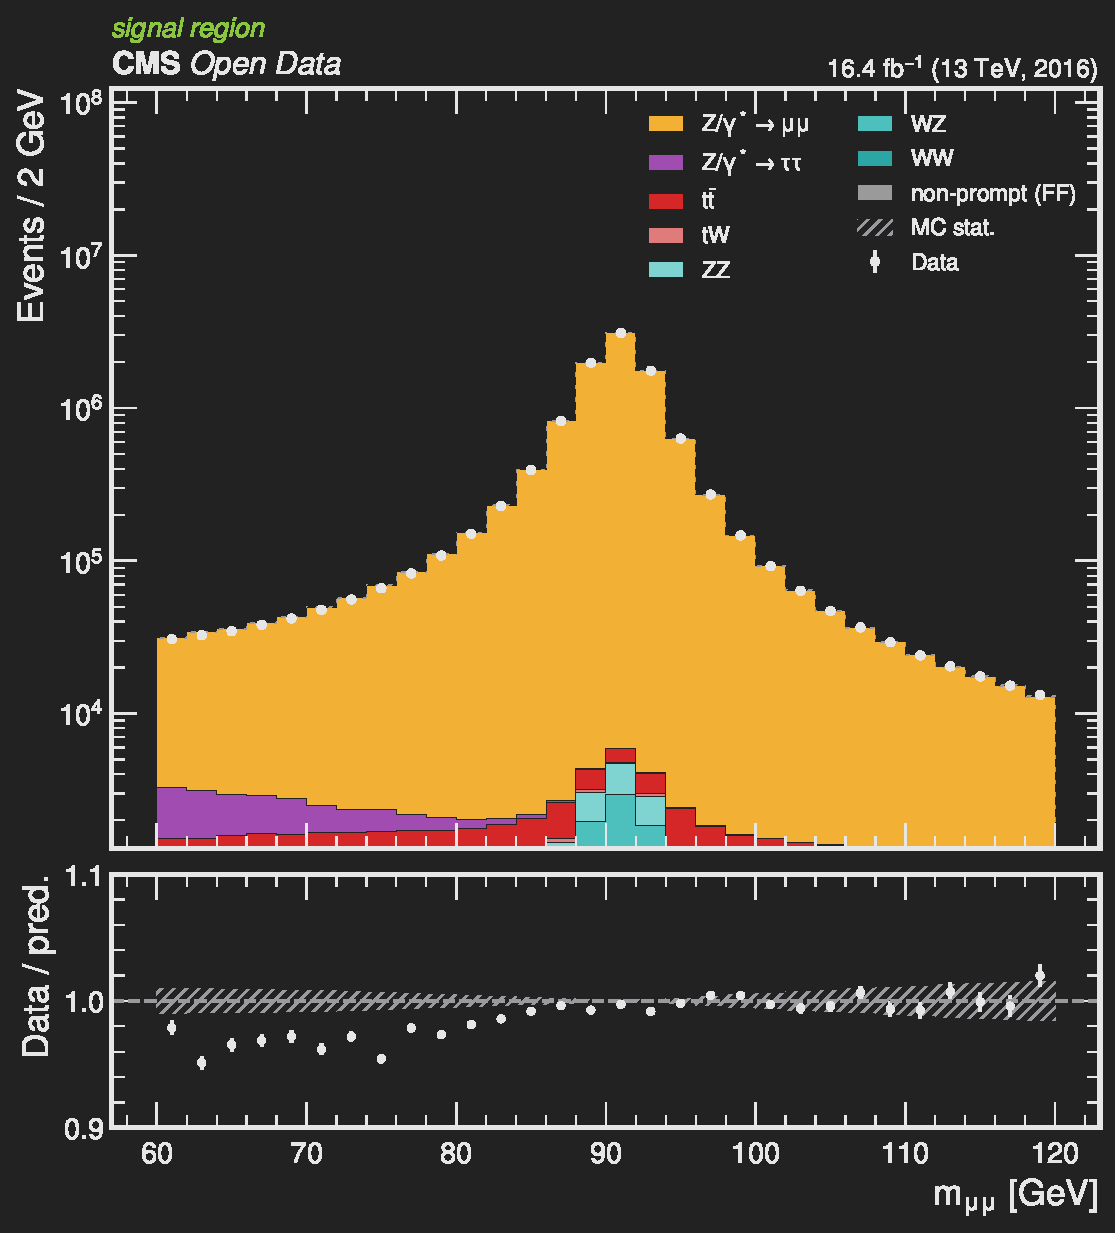
\includegraphics[height=0.7\textheight]{sr_mass_log.pdf}\end{column}
  \end{columns}
  \fcap{10\,378\,567 data events; prompt MC + fake factor 10\,445\,834 pre-fit. The 3--4\,\% deficit at 62--78 GeV (left ratio) is what drives F3.}
\end{frame}

\begin{frame}{Tag-and-probe: trigger and identification}
  \centering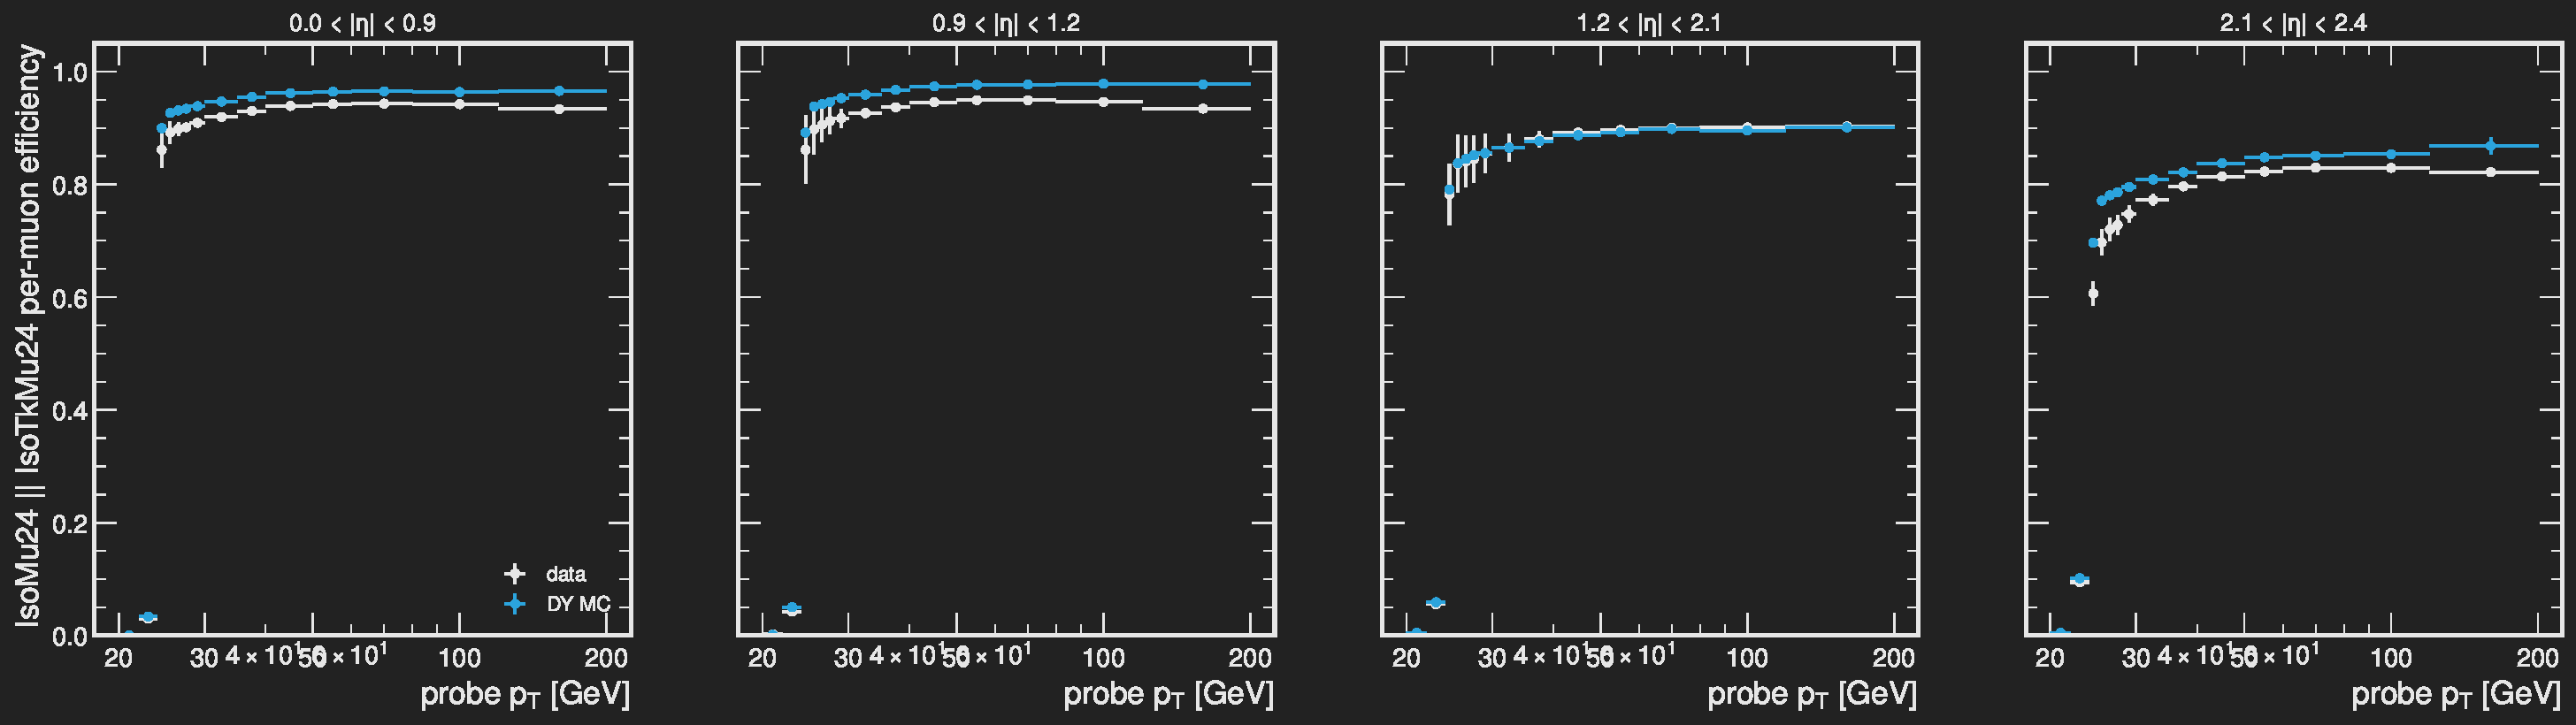
\includegraphics[height=0.36\textheight]{tnp_trigger.pdf}\\[0.05cm]
  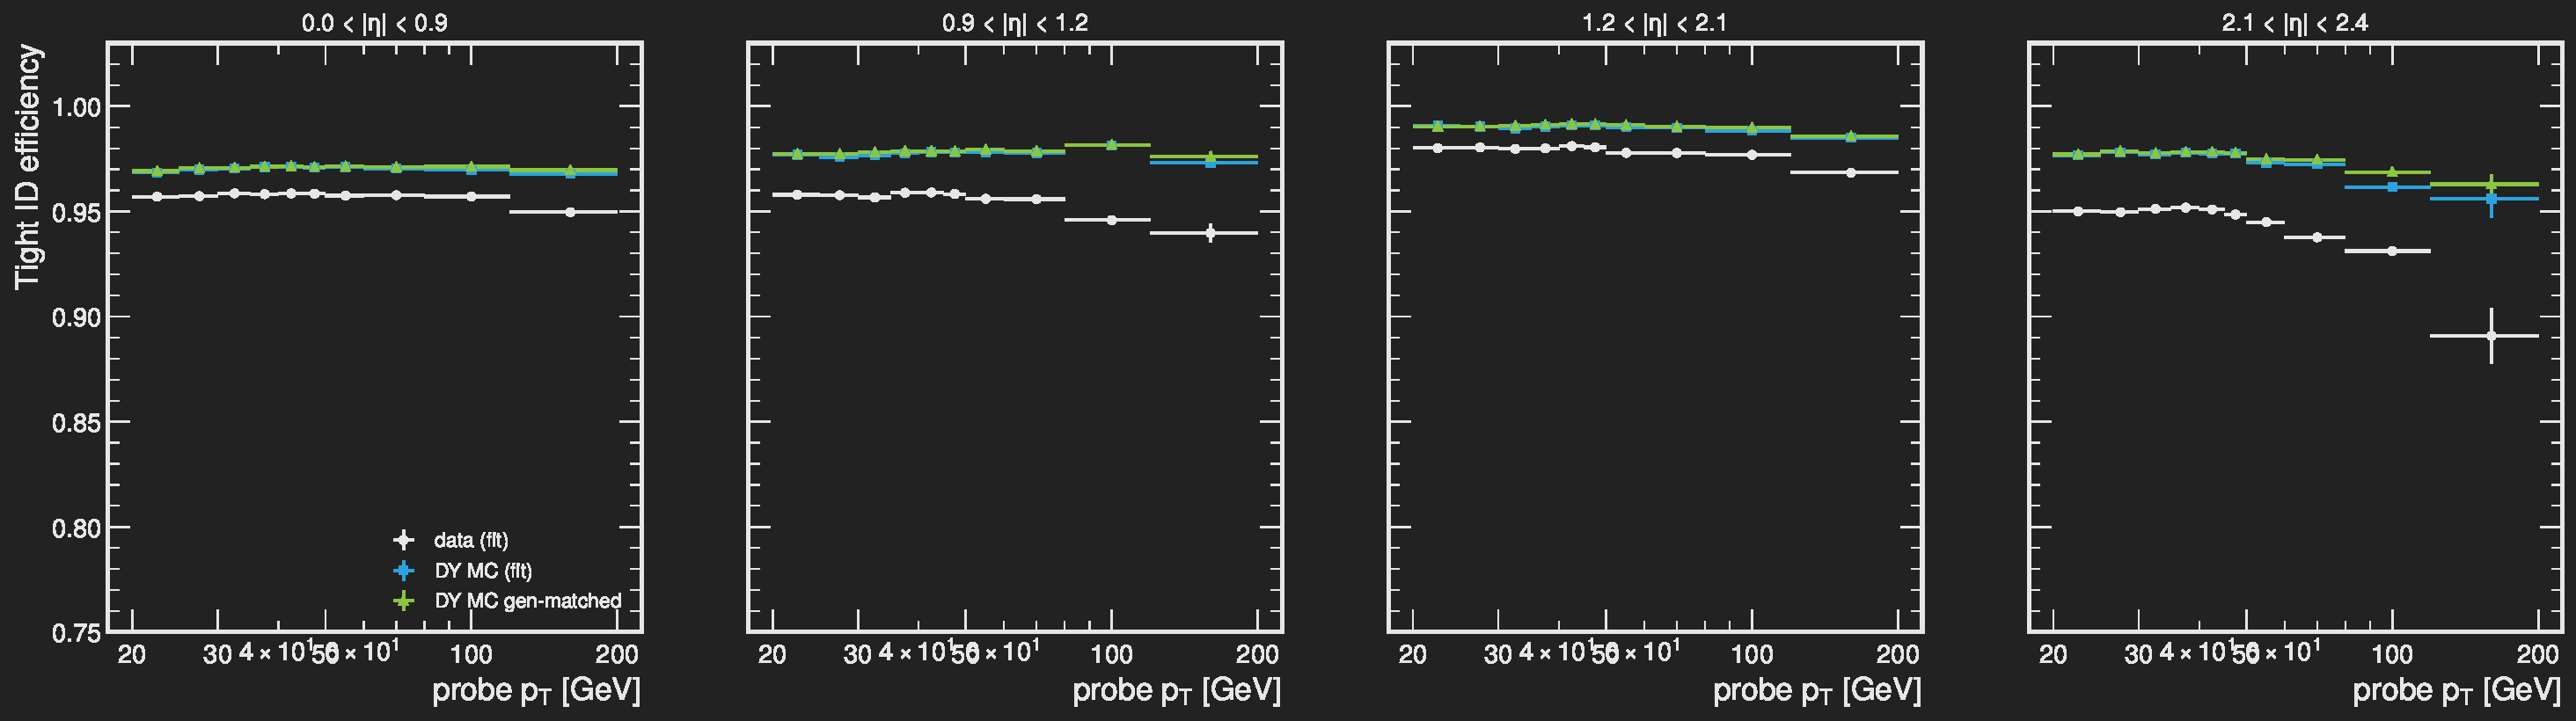
\includegraphics[height=0.36\textheight]{tnp_eff_id.pdf}
  \fcap{Trigger-object T\&P (top; plateau 0.907 data / 0.923 MC per muon) and tight-ID pass/fail fits (bottom; closure to gen-matched truth $-$0.1\,\%). Sound.}
\end{frame}

\begin{frame}{Tag-and-probe: scale-factor maps}
  \begin{columns}[T]
    \begin{column}{0.49\textwidth}\centering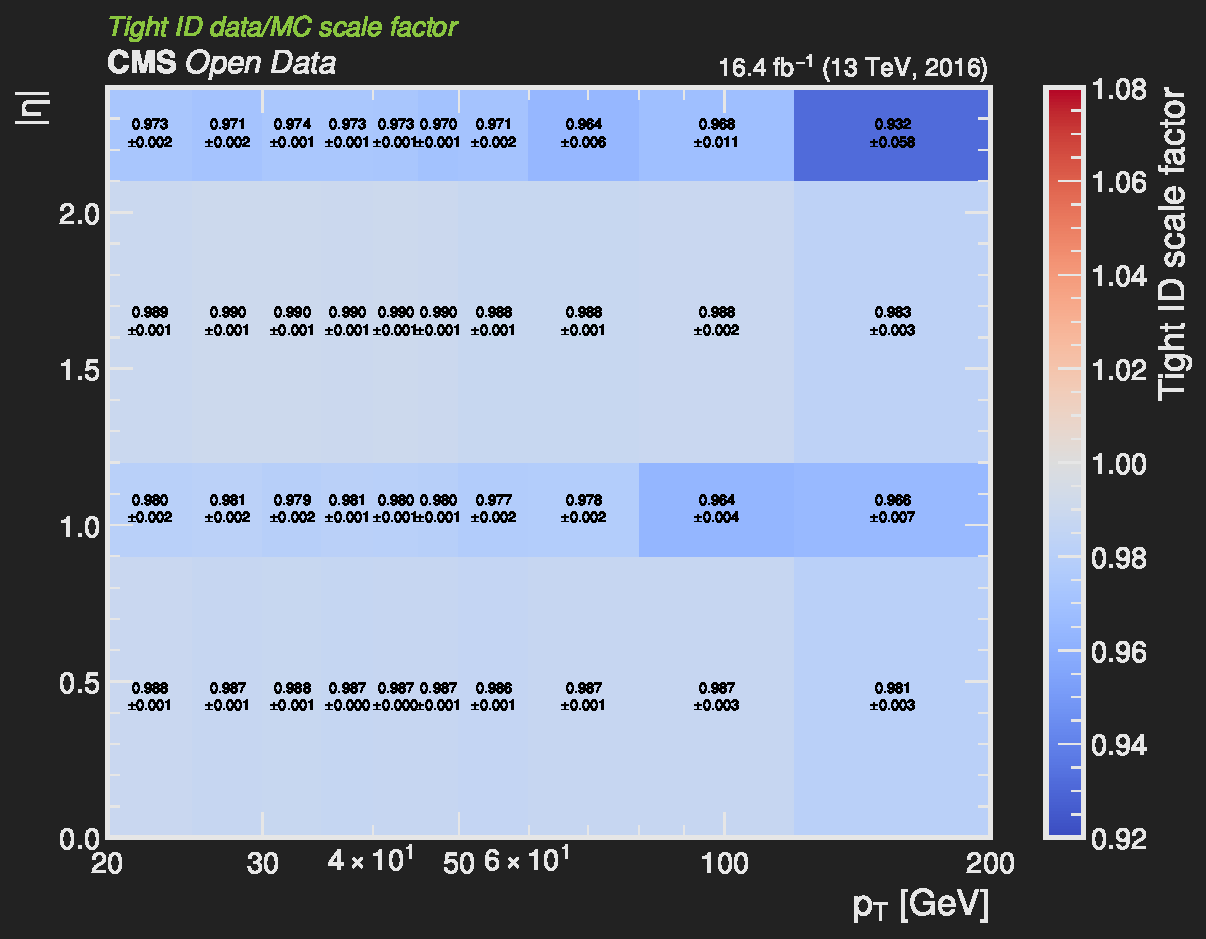
\includegraphics[width=\textwidth]{tnp_sf_id_map.pdf}\fcap{tight ID: 0.97--0.99, $\langle\mathrm{SF}\rangle$ = 0.980 $\pm$ 0.0014 (stat) $\pm$ 0.0029 (syst)}\end{column}
    \begin{column}{0.49\textwidth}\centering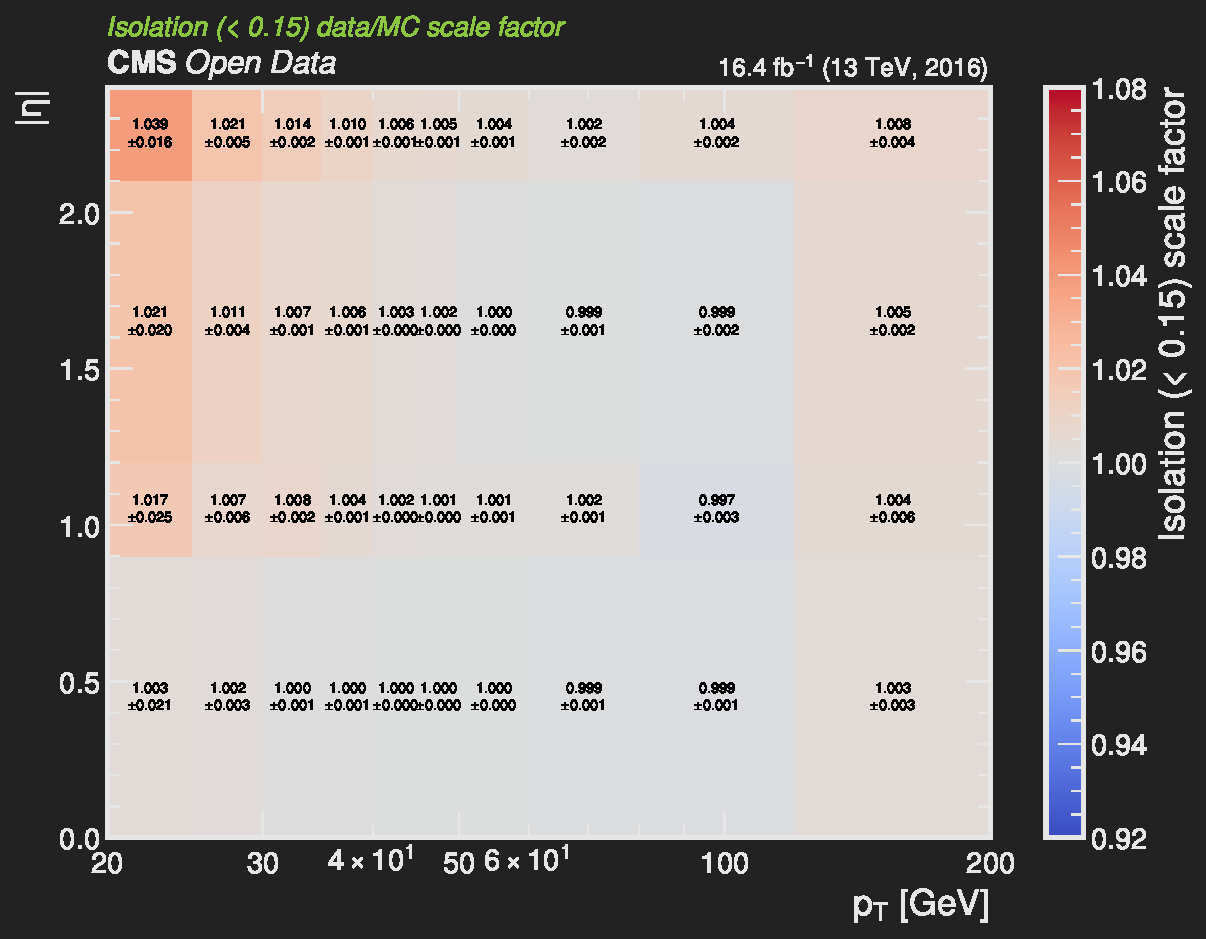
\includegraphics[width=\textwidth]{tnp_sf_iso_map.pdf}\fcap{isolation: 1.00--1.04, $\langle\mathrm{SF}\rangle$ = 1.005; flat in pileup (half-spread 0.0024)}\end{column}
  \end{columns}
  \small The \texttt{MuonIso} variation is applied coherently to all cells; its shape ($+1.1$\,\% at 60 GeV, $+0.2$\,\% at 120 GeV) is what the fit exploits when \texttt{SigModel} is absent (F3).
\end{frame}

\begin{frame}{Fake factor and momentum calibration}
  \centering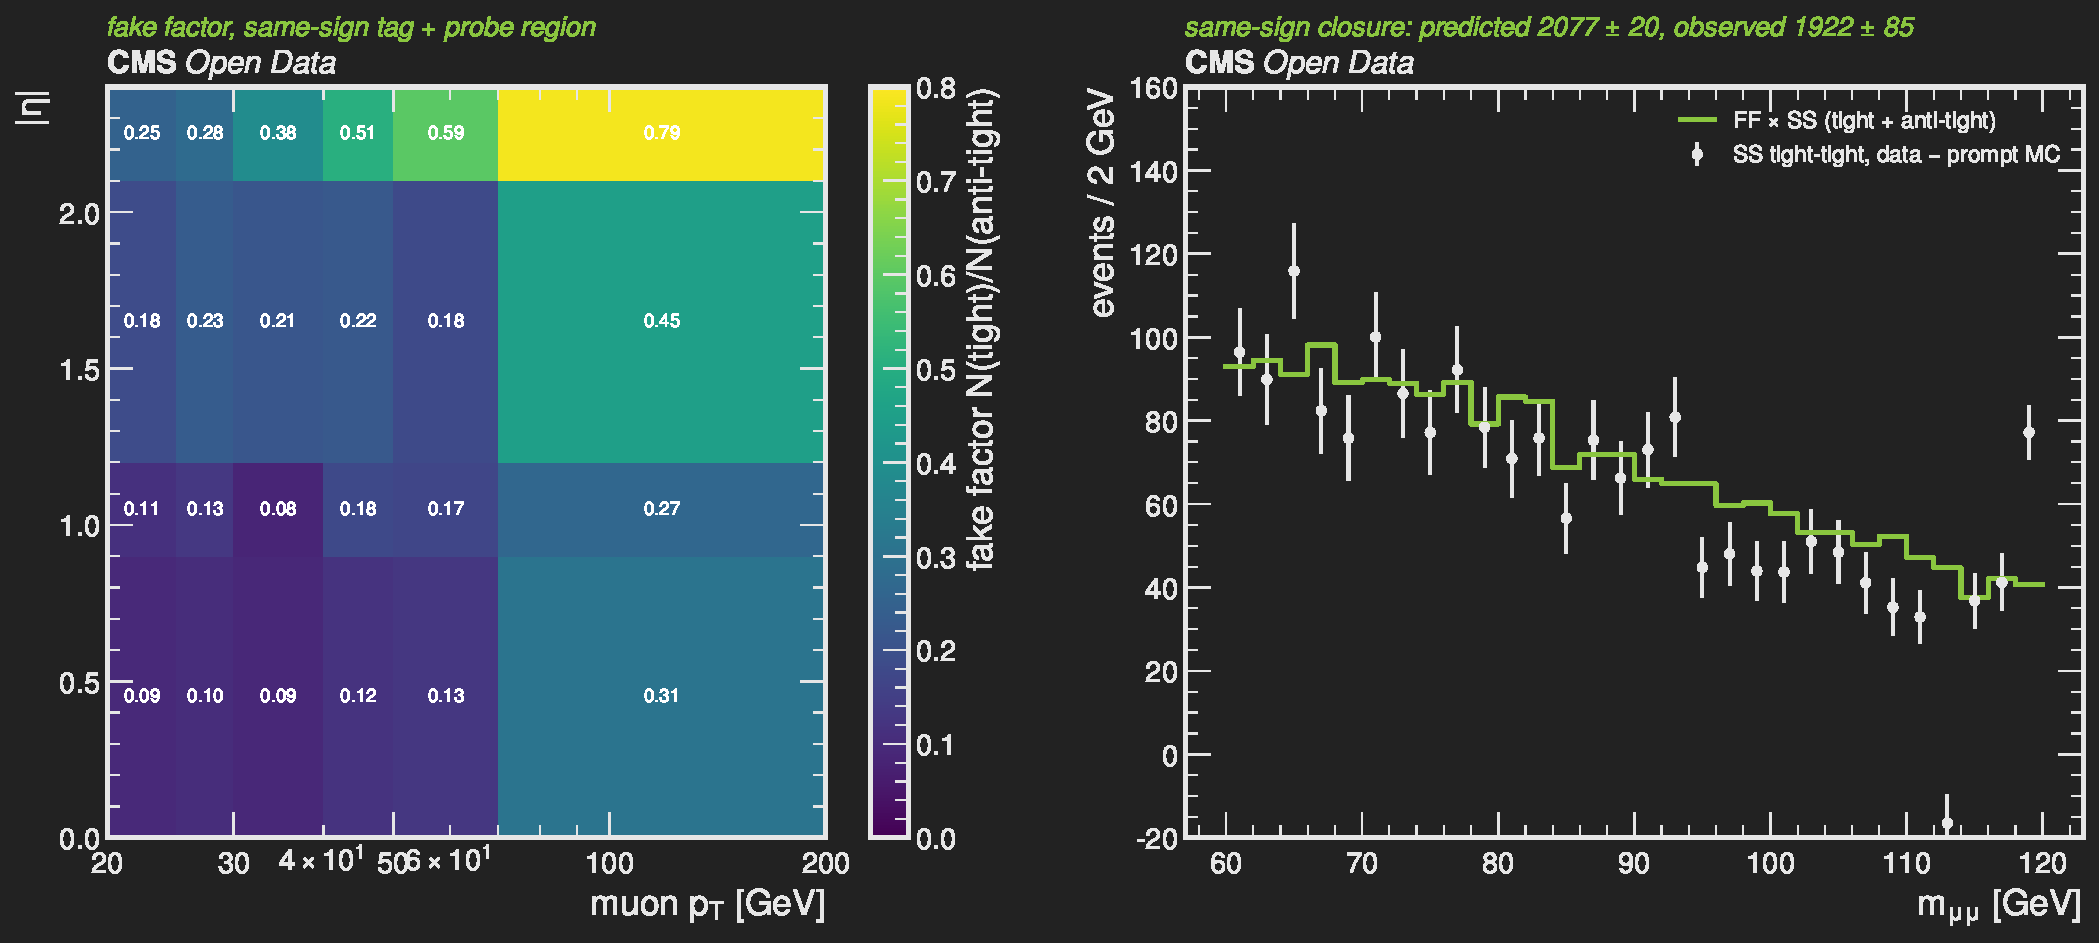
\includegraphics[height=0.42\textheight]{ff_map_and_closure.pdf}\\[0.05cm]
  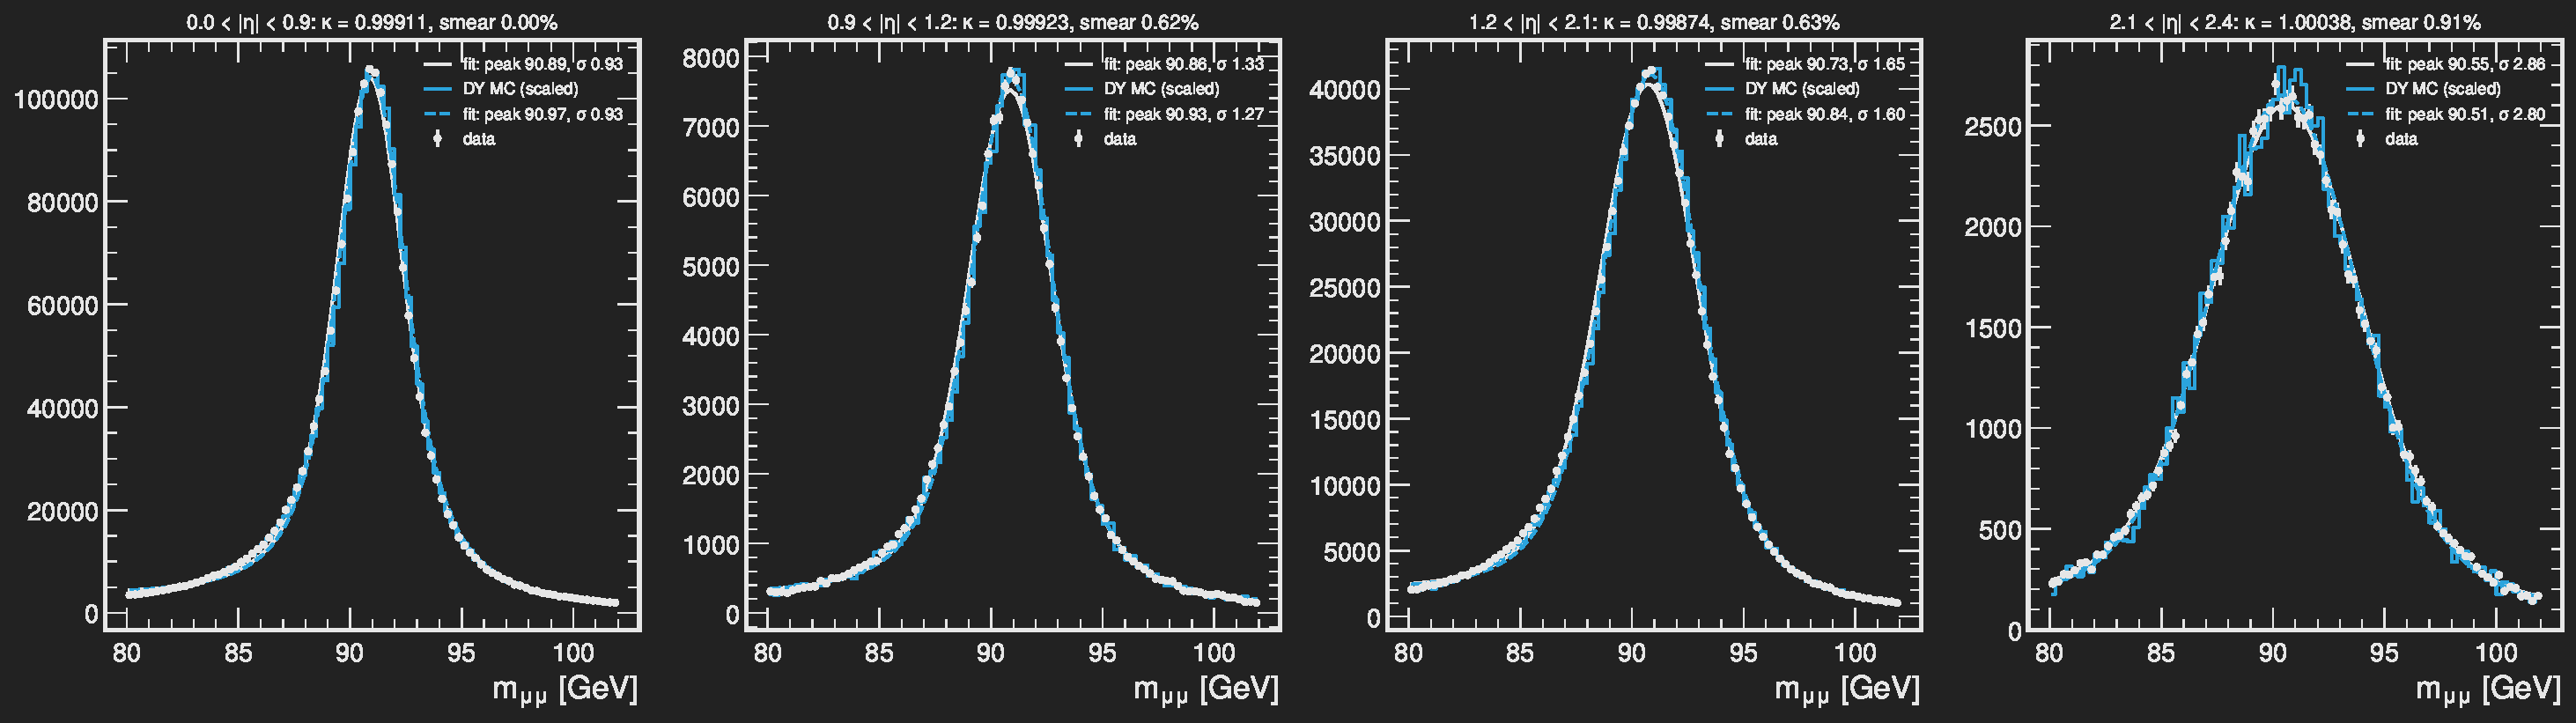
\includegraphics[height=0.28\textheight]{momentum_zpeak.pdf}
  \fcap{Fake factor (SS tag+probe, prompt-subtracted): SR non-prompt 3\,825 $\pm$ 80 (stat) $\pm$ 30\,\% (method), closure 2077 $\pm$ 20 vs 1922 $\pm$ 85. Momentum: $\kappa$ and extra smearing per $|\eta|$; then used again as \texttt{MuonScale}/\texttt{MuonRes} in the fit.}
\end{frame}

% ================================================================= 5. choices and recommendations
\divider{Choices reviewed, recommendations}

\begin{frame}{Analysis choices: verdicts}
  \tsize
  \begin{tabular}{L{5.6cm}L{1.9cm}L{5.6cm}}
    \thead choice & verdict & comment\\
    \rowcolor{rowA} tight ID + iso $<$ 0.15, IP cuts; dressed fiducial volume & \bestcell{good} & matches the external reference; dressed avoids the 1.8\,\% Born ambiguity\\
    \rowcolor{rowB} own skims; normtag luminosity; L1 prefiring weight & \bestcell{good} & prefiring not double counted by the T\&P (prefired events never enter)\\
    \rowcolor{rowA} T\&P with pass/fail fits, trigger-matched tag, per-event trigger weight & \bestcell{good} & closure $-$0.1/$-$0.2\,\%; $\chi^2/$ndf $\approx$ 2 in data covered by variants\\
    \rowcolor{rowB} fake factor from SS tag+probe; single-$\mu$+jet region rejected & \bestcell{good} & template fit handles the Z-dominated anti-isolated sample\\
    \rowcolor{rowA} Z-peak momentum calibration & good & but the same peak then constrains the NPs to 0.1$\sigma$ (used twice)\\
    \rowcolor{rowB} pileup profile from the luminosity CSV & stop-gap & 4\,\% low, no bunch spread (F6)\\
    \rowcolor{rowA} prompt-prompt MC in SR/SS (0.006\,\% loss, FF replaces) & \bestcell{good} & \\
    \rowcolor{rowB} prompt-prompt MC in the e$\mu$ region, no replacement & \warncell{wrong} & F1\\
    \rowcolor{rowA} theory variations renormalised to constant fiducial yield & \bestcell{good} & correct for a fiducial measurement\\
    \rowcolor{rowB} 30 $\times$ 2 GeV shape fit with 24 NPs + 30 gammas & \warncell{not robust} & F3/F5\\
    \rowcolor{rowA} powheg \texttt{SigModel} one-sided template & \warncell{wrong as built} & F4\\
    \rowcolor{rowB} e$\mu$ as VALIDATION; NLO acceptance, 60--120 denominator & \bestcell{good} & keep VALIDATION until F1 is fixed\\
    \rowcolor{rowA} jets not lepton-cleaned in the plots & bug & F7\\
  \end{tabular}
\end{frame}

\begin{frame}{Recommendations, by impact}
  \small
  \begin{enumerate}
    \item \textbf{Signal extraction (F3--F5).} Rebuild \texttt{SigModel} with the same LHE mass window on both generators; understand the 62--78 GeV deficit (generator-level lineshapes, unfolded data); until then quote the counting extraction ($794.4$ pb) with a $\pm$0.7\,\% lineshape term, keep the 30-bin fit as a cross-check. If a shape fit is kept: coarse bins, consistent smoothing, external \texttt{Lumi} (1.2\,\%), pre-fit values for \texttt{Pileup}/\texttt{MuonIso}.
    \item \textbf{e$\mu$ region (F1).} Keep the non-prompt MC or use the same-sign estimate; add the SS e$\mu$ region to \texttt{regions.py} and the plots. Then the flavour-symmetric backgrounds are validated to $\sim$2\,\% (0.01\,\% on $\sfid$).
    \item \textbf{\texttt{MuonReco} (F8).} Per muon or per event: fix the config or the documentation (+0.35\,\% in quadrature if per muon).
    \item \textbf{Pileup (F6).} $N_{PV}$-matched profile or the official JSON; re-check the \texttt{Pileup} pull.
    \item \textbf{Jets (F7).} $\Delta R(\mathrm{jet},\ell) > 0.4$ cleaning in \texttt{histograms.py}.
    \item $\met$: nothing for $\mu\mu$; JER smearing or Puppi $\met$ + \texttt{MET\_Unclustered} wherever $\met$ is cut on (relevant for the $\tau\tau$ channel, which shares these conventions).
    \item Z $p_T$ reweighting or an explicit NP (enters $C$ via the $p_T$ thresholds at 0.1--0.2\,\%).
  \end{enumerate}
  \vspace{0.2cm}
  \textbf{For the combination:} use $\sfid = 794.4$ pb (counting) or the fit value with the extra 0.7\,\% until item 1 is done; the correlated NP names and the acceptance convention (NLO, $60<m<120$) are fine as they stand.
\end{frame}

% ================================================================= 6. backup
\divider{Backup}
\greentitles

\begin{frame}{Backup: same-sign e$\mu$ region}
  \centering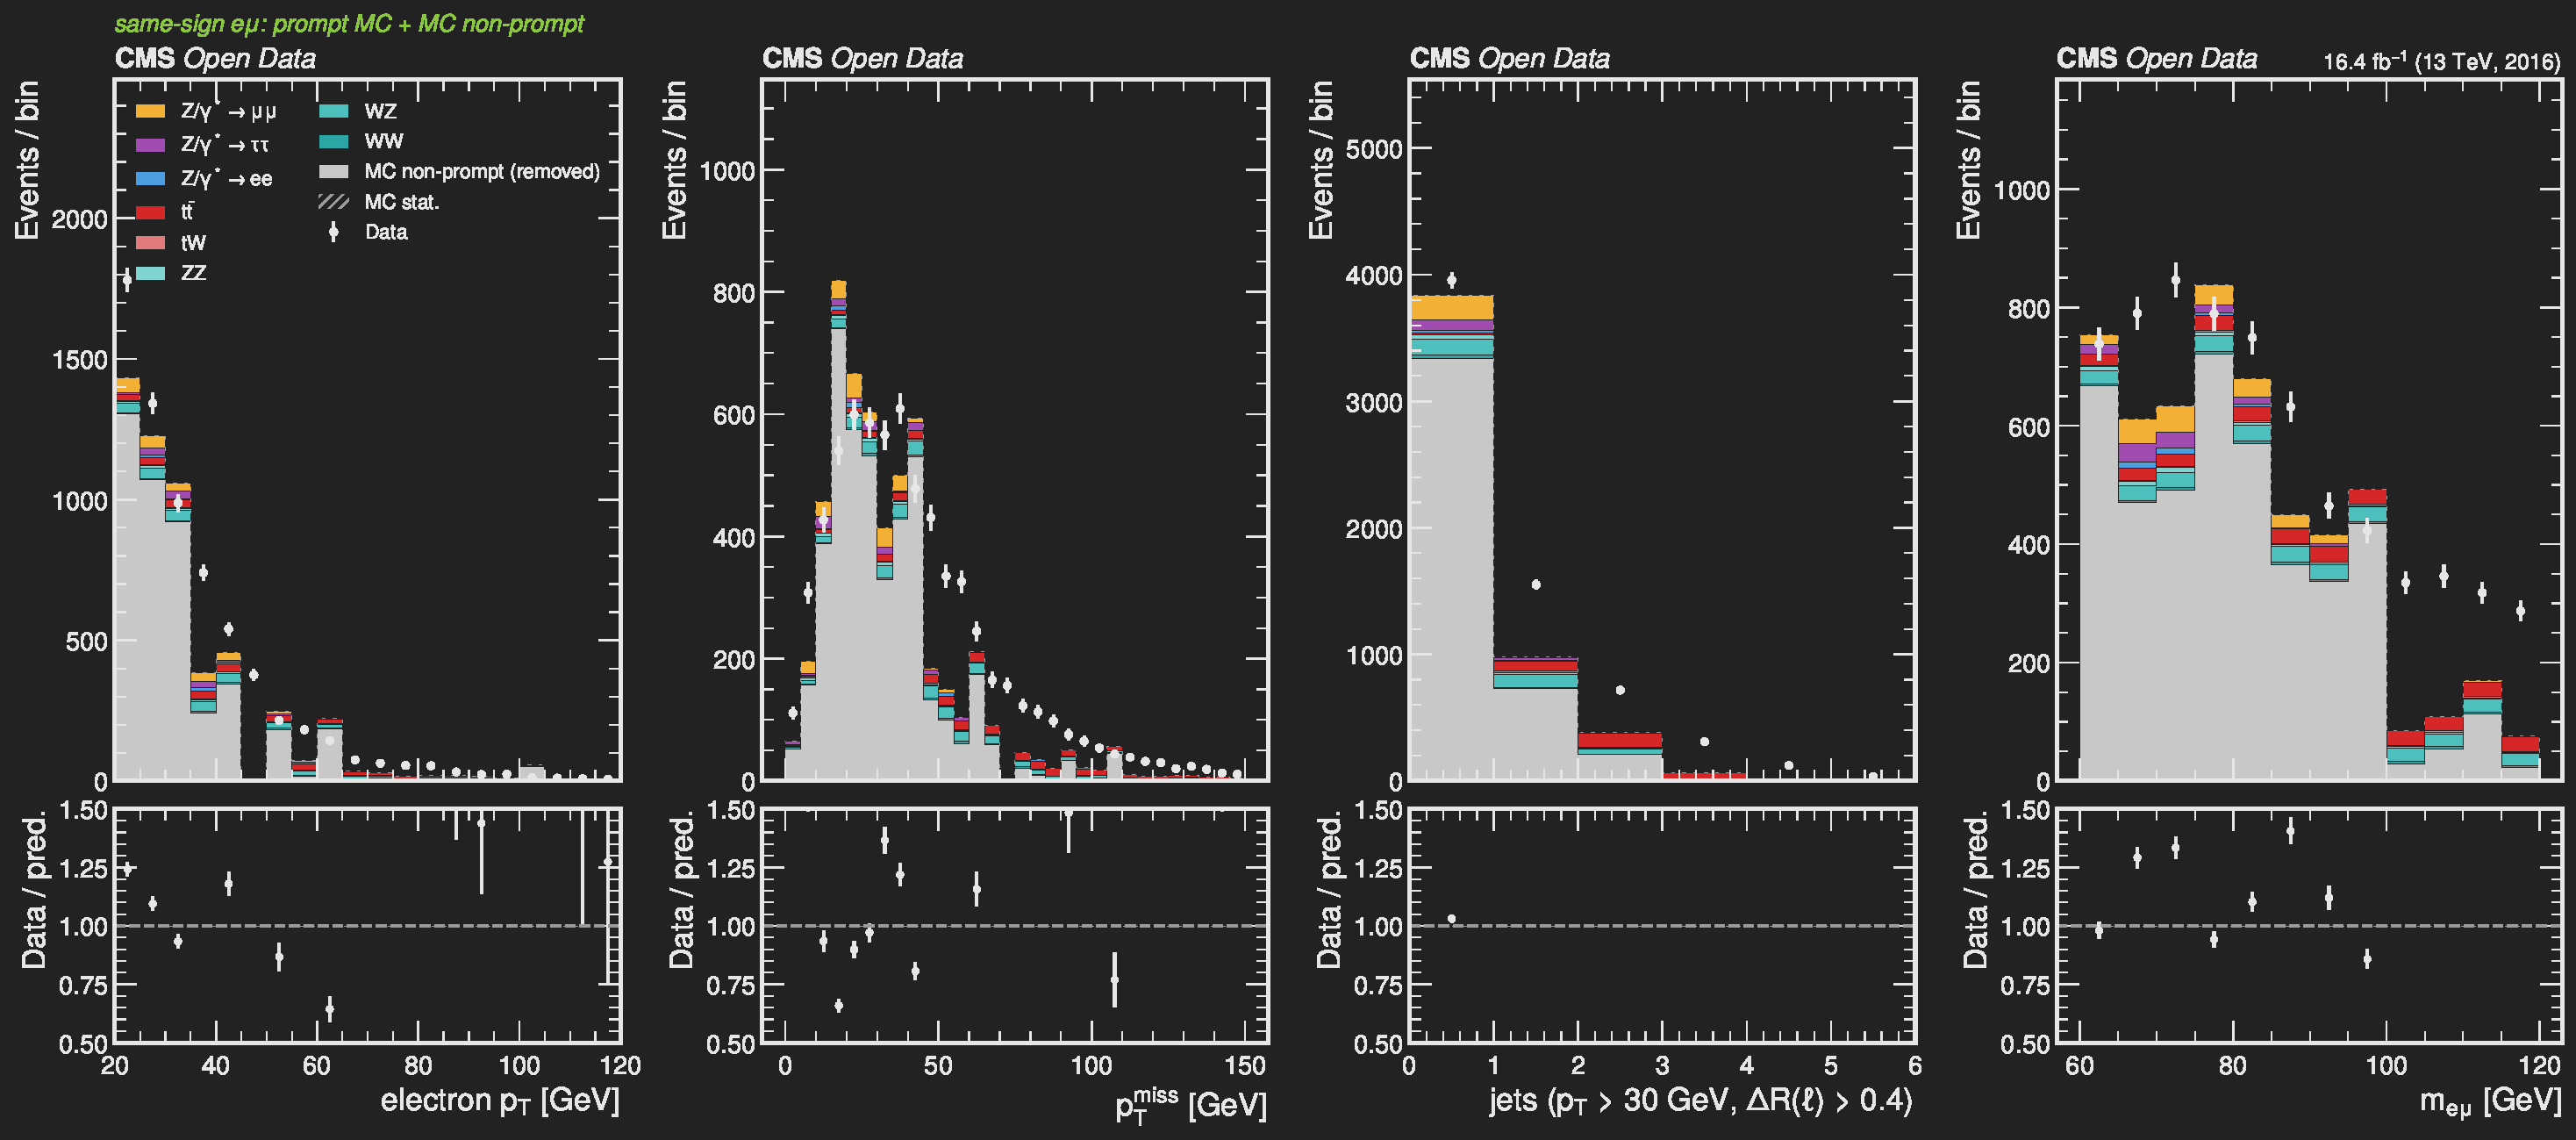
\includegraphics[width=0.97\textwidth]{emu_ss.pdf}
  \fcap{Same-sign e$\mu$: 6\,718 data, 1\,039 prompt MC, 4\,275 MC non-prompt. The MC underestimates the SS region by 26\,\% (no QCD sample, tiny W+jets skim): the data-driven SS number is the reliable one.}
\end{frame}

\begin{frame}{Backup: the jet-multiplicity bug and other SR distributions}
  \begin{columns}[T]
    \begin{column}{0.33\textwidth}\centering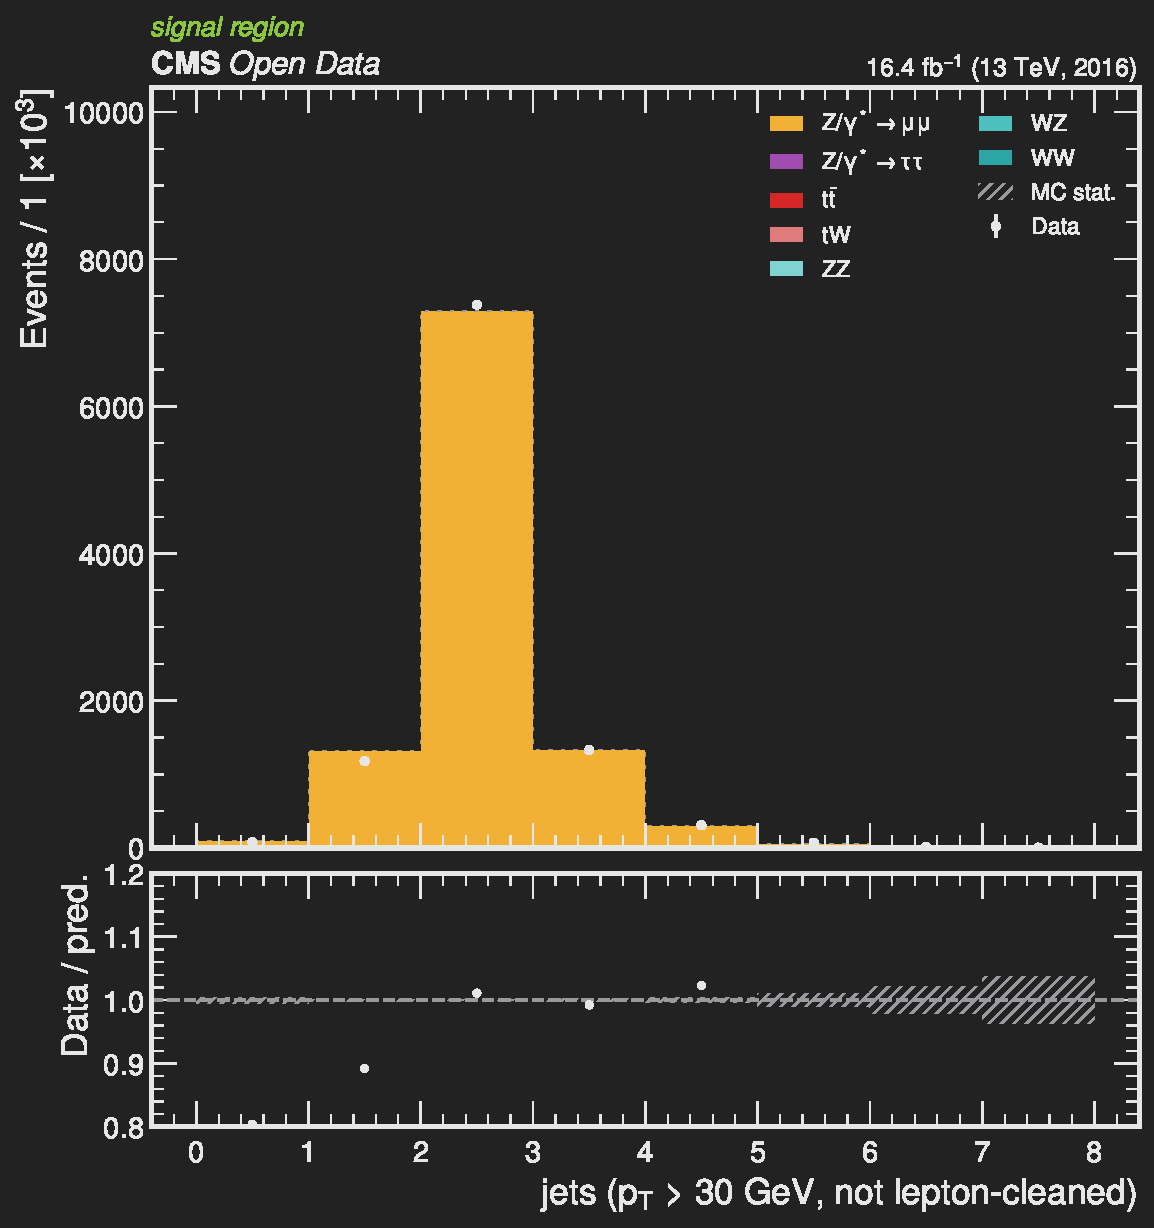
\includegraphics[height=0.6\textheight]{sr_njet.pdf}\fcap{``jets'' peak at 2: the two muons are counted (F7)}\end{column}
    \begin{column}{0.33\textwidth}\centering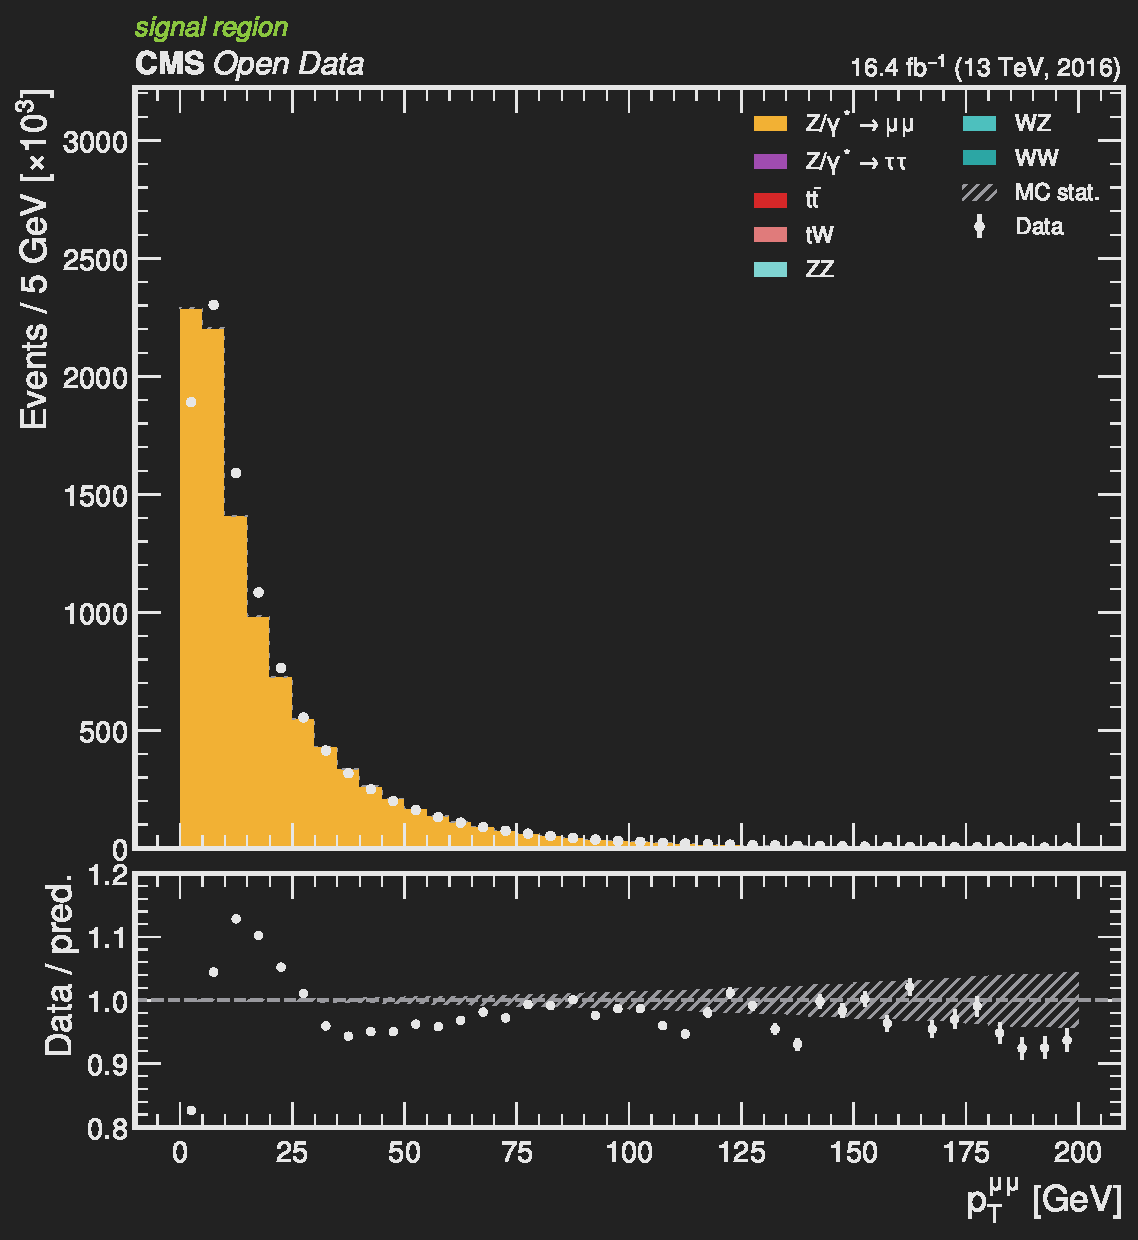
\includegraphics[height=0.6\textheight]{sr_zpt.pdf}\fcap{Z $p_T$: 0.83 at 0--5 GeV, 1.13 at 10--15 GeV}\end{column}
    \begin{column}{0.33\textwidth}\centering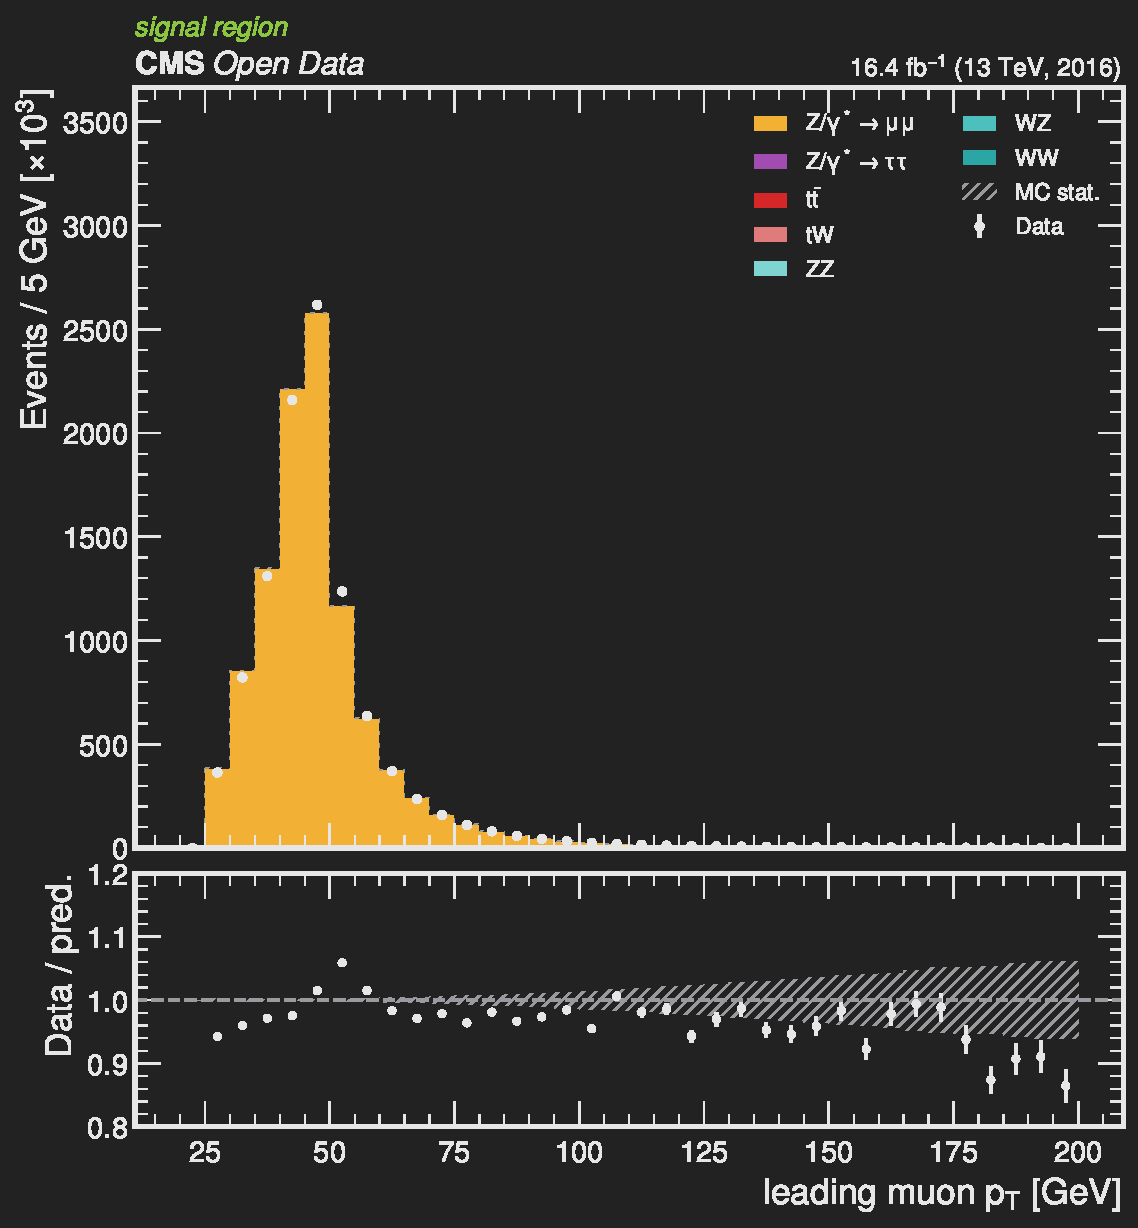
\includegraphics[height=0.6\textheight]{sr_pt1.pdf}\fcap{leading muon $p_T$}\end{column}
  \end{columns}
\end{frame}

\begin{frame}{Backup: same-sign $\mu\mu$ and e$\mu$ jets}
  \begin{columns}[T]
    \begin{column}{0.33\textwidth}\centering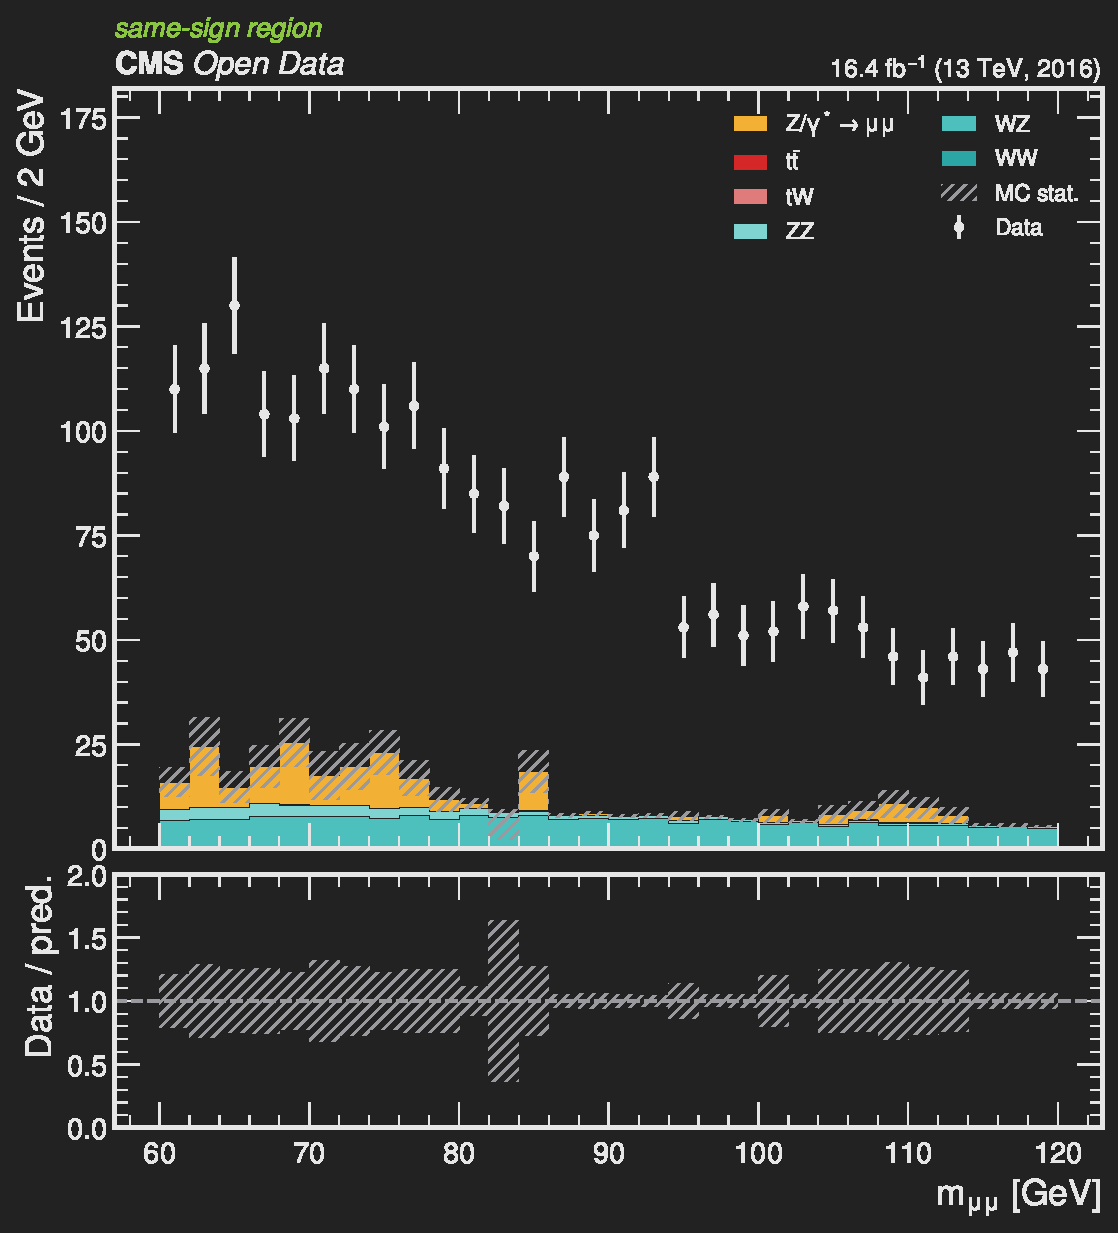
\includegraphics[height=0.6\textheight]{ss_mass.pdf}\fcap{SS $\mu\mu$: prompt MC only; the rest is the non-prompt background (fake-factor closure region)}\end{column}
    \begin{column}{0.33\textwidth}\centering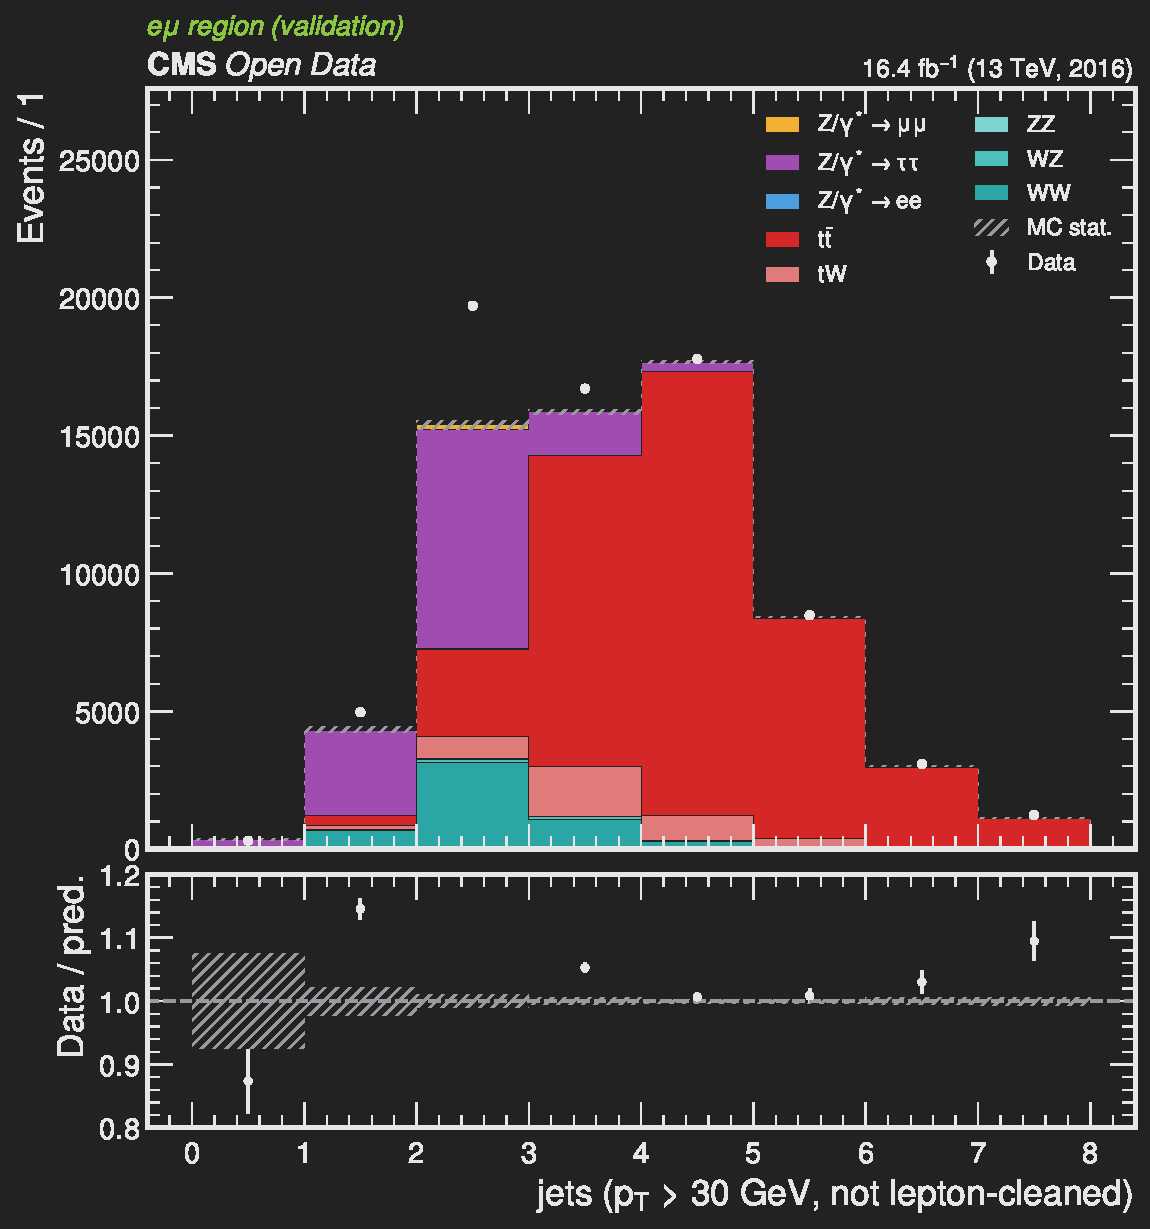
\includegraphics[height=0.6\textheight]{cr_njet.pdf}\fcap{e$\mu$ ``jets'' (not cleaned): the excess sits in the bins with no real jet}\end{column}
    \begin{column}{0.33\textwidth}\centering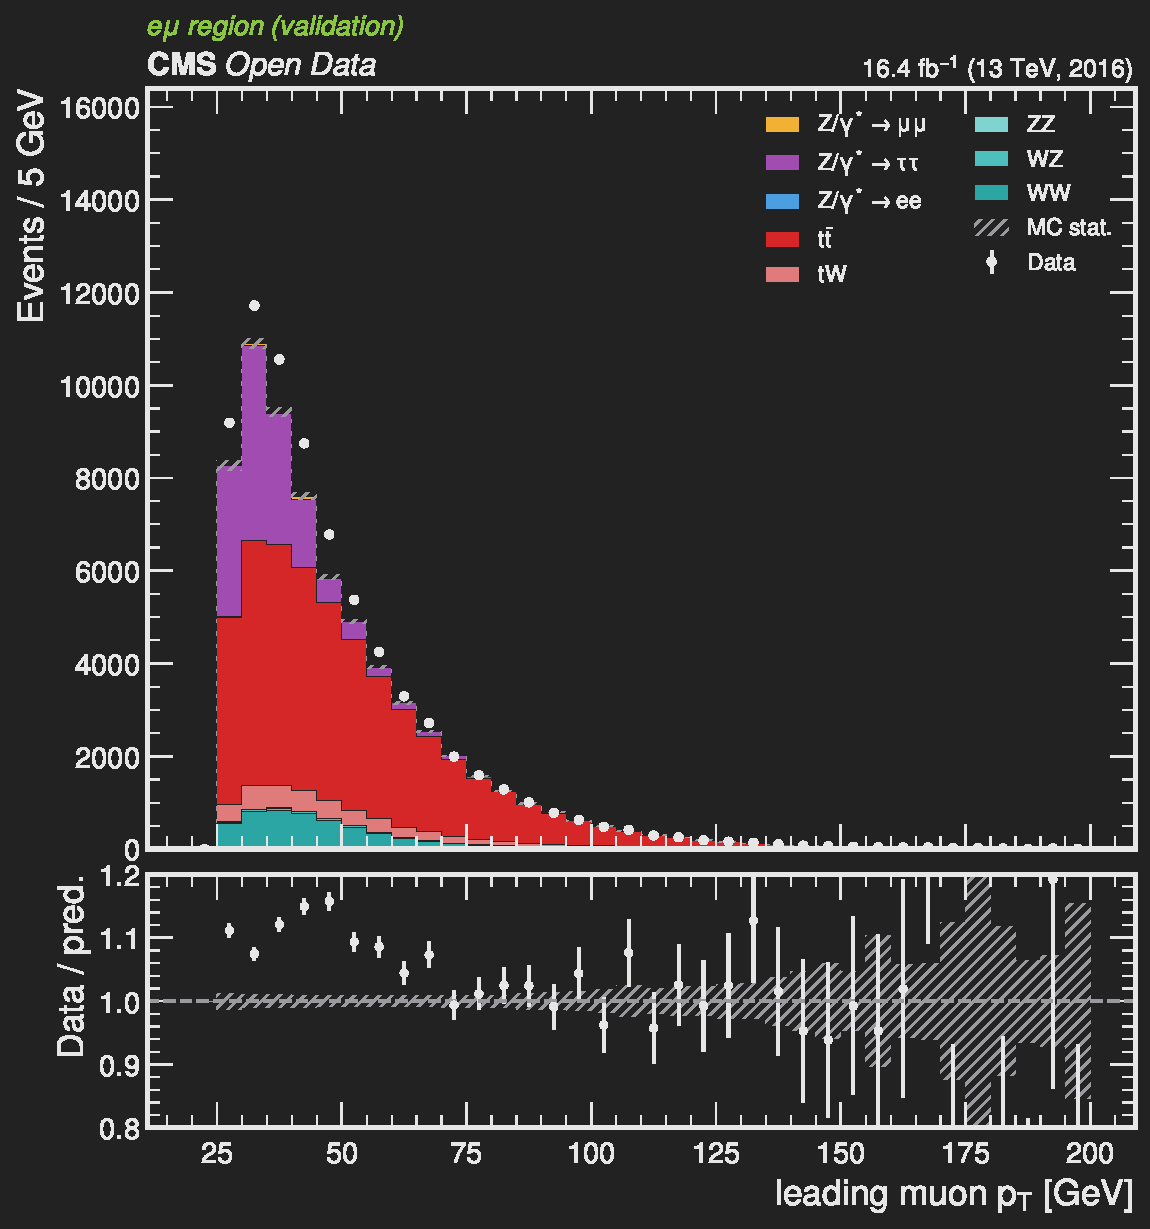
\includegraphics[height=0.6\textheight]{cr_pt1.pdf}\fcap{e$\mu$: leading muon $p_T$}\end{column}
  \end{columns}
\end{frame}

\begin{frame}{Backup: isolation efficiency}
  \centering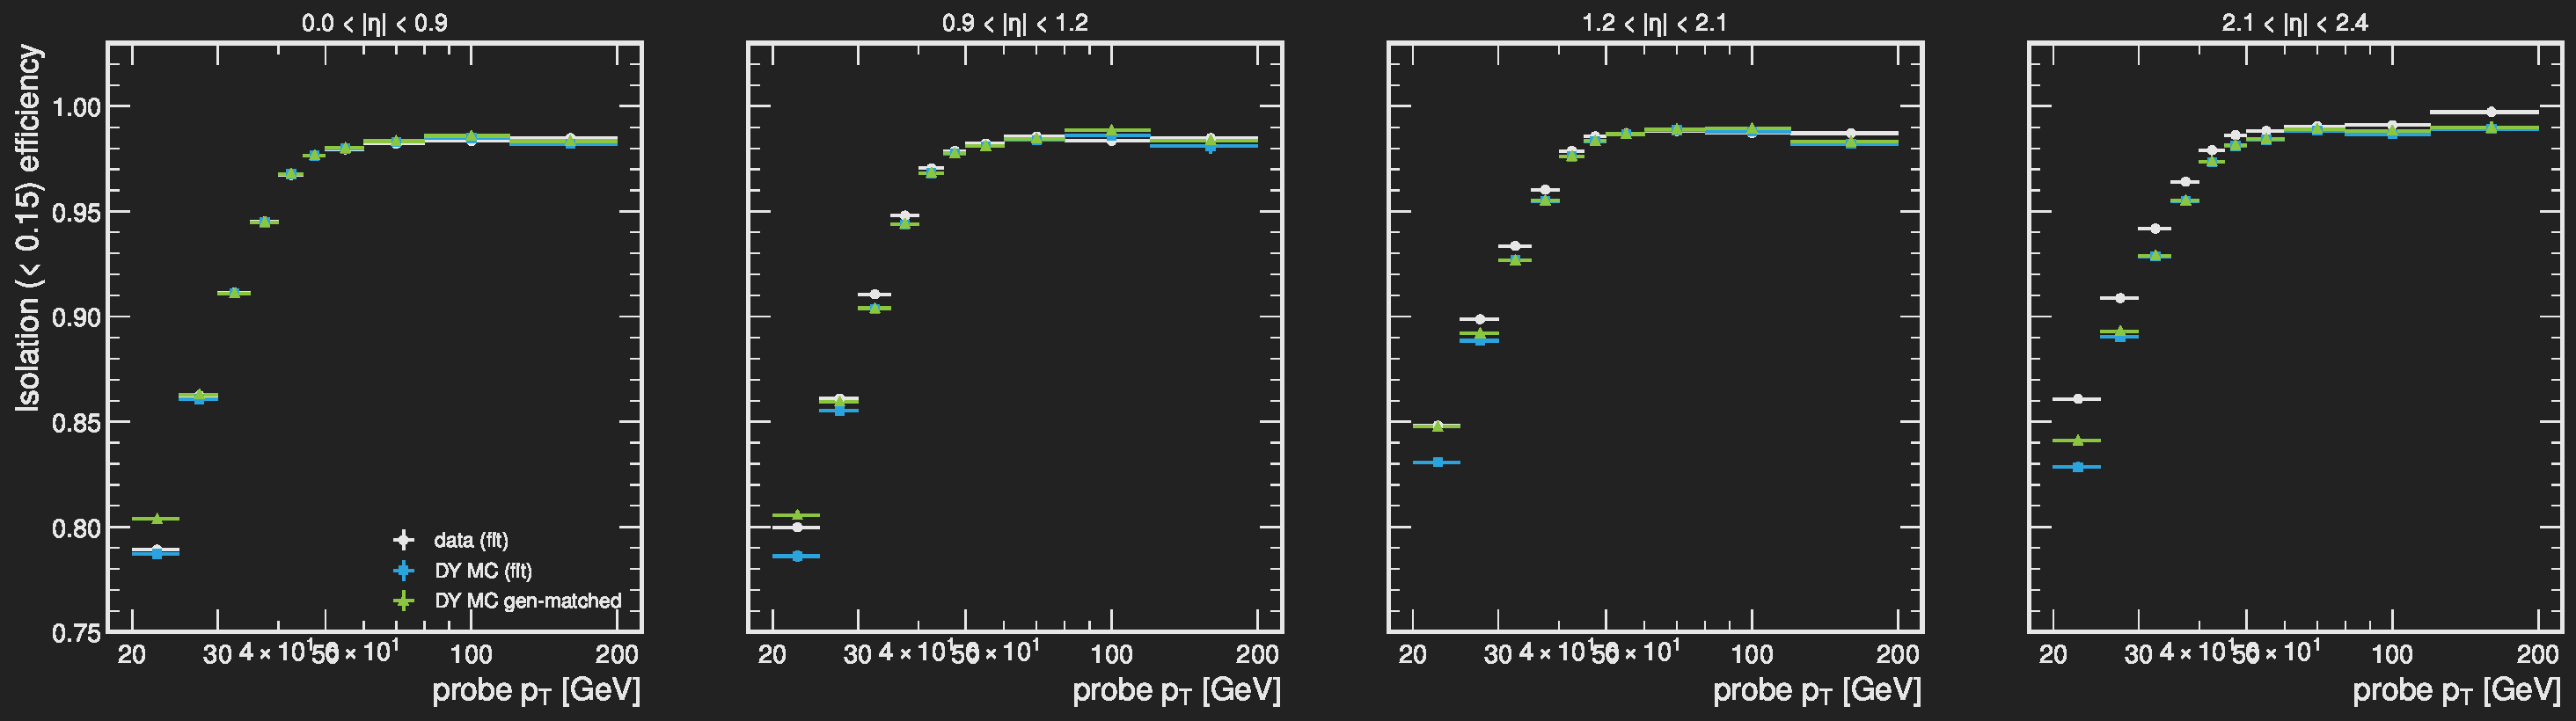
\includegraphics[width=0.97\textwidth]{tnp_eff_iso.pdf}
  \fcap{Isolation efficiency vs probe $p_T$, data and MC fits and gen-matched truth; the fit-vs-truth closure is $-$0.2\,\%.}
\end{frame}

\end{document}
